% This is LLNCS.DEM the demonstration file of
% the LaTeX macro package from Springer-Verlag
% for Lecture Notes in Computer Science,
% version 2.4 for LaTeX2e as of 16. April 2010
%
\documentclass{llncs}
%
\usepackage{makeidx}  % allows for indexgeneration
%
\usepackage{todonotes}
%


\usepackage{booktabs}
\usepackage{graphicx}
\usepackage{amssymb}
\usepackage{color}

% http://mirror.utexas.edu/ctan/obsolete/macros/latex/contrib/subfigure/subfigure.pdf
\usepackage[tight]{subfigure}

\begin{document}
%
\frontmatter          % for the preliminaries
%
\pagestyle{headings}  % switches on printing of running heads
\addtocmark{Alpha Shapes for Tumor Inclusion} % additional mark in the TOC
%

%
%\tableofcontents
%
%\listoftodos

\mainmatter              % start of the contributions
%
\title{Lung Segmentation via Alpha Shapes in the Presence of Large Tumors}
%
\titlerunning{Alpha Shape Lung Segmentation}  % abbreviated title (for running head)
%                                     also used for the TOC unless
%                                     \toctitle is used
%
\author{I.M. Anonymous\inst{1}\\
\and U.R. Anonymous\inst{2}
}
%\author{
%Sarah E. Gerard\inst{1,3} \and
%Hans J. Johnson\inst{1,3} \and
%John E. Bayouth\inst{2} \and\\
%Kaifang Du\inst{2} \and
%Junfeng Guo\inst{1,3} \and
%Joseph M. Reinhardt\inst{1,3}
%}
%
\authorrunning{Sarah E. Gerard et al.} % abbreviated author list (for running head)
%
%%%% list of authors for the TOC (use if author list has to be modified)
\tocauthor{Sarah E. Gerard, Hans J. Johnson, John E. Bayouth, Kaifang Du, Junfeng Guo, Joseph M. Reinhardt}
%
\institute{
Nowhere \and
Noplace \and
Nowhere 
}
%\institute{
%University of Iowa, USA 
%\and University of Wisconsin-Madison, USA
%\and Iowa Institute for Biomedical Imaging 
%}


\maketitle              % typeset the title of the contribution

\todo[author=SG]{You are not doing just "lung segmentation" it is "lung cavity segmentation" that includes both lung tissue and included tumors.  Can you clarify this in the abstract to make more clear that you are capturing BOTH lung and included tumors?}

\begin{abstract}
\textcolor{red}{Lung segmentation} is a critical initial step in planning radiation therapy interventions for lung cancer patients. Achieving robust automatic segmentation of lungs with large tumors is challenging due to large variations in lung morphology, tumor location, and tumor shape between subjects. We present an automatic method to \textcolor{red}{segment lungs} with large tumors in CT images using an initial intensity based segmentation followed by alpha shape construction and graph search. We evaluated our method by comparing automated segmentations to manual segmentations on twelve subjects. Computed metrics for segmentation quality include average surface distance of 0.727 and average DICE coefficient of 0.970. These results demonstrate that the proposed method accurately segments the entire lung regions both absent of and in the presence of large tumors. 
\keywords{segmentation, alpha shape, lung, radiation therapy}
\end{abstract}
%
\section{Introduction}
%
Radiation therapy interventions of lung cancer patients involve acquiring a thoracic CT scan to assess the disease state and to design a patient specific treatment plan. Typically a respiratory correlated scan, or 4D CT, is also acquired prior to treatment. This produces a huge amount of data, requiring automatic computer-aided methods for further analysis. Accurate delineation of the lungs is a critical initial first step for treatment planning and quantitative analysis.

Normal lung tissue has high contrast with the surrounding anatomy, making lung segmentation relatively robust using simple thresholding based methods~\cite{guo2008,hu2001}. However, in the presence of large tumors, conventional threshold based methods fail because the radiodense tumors are excluded from the segmentation. An accurate lung tissue segmentation inclu is required during radiation therapy planning, e.g., to predict the dose delivered to the normal lung tissue and the tumor. 

Several approaches have been used to segment pathological lungs. Statistical shape models (SSM) have bee used to capture the major modes of lung shape variation in a training set used to build a lung model~\cite{sofka2011,sun2012}. The SSM method, however, requires a large training set with annotated manually identified corresponding landmark points. Additionally, the SSM training set is limited to a subset of possible lung shape variations and thus it often fails on cases that are not represented in the training set. Segmentation by registration methods~\cite{sluimer2005,vanrikxoort2009} make use an atlas or multiple atlases with ground truth segmentations. The atlas segmentation is mapped to a test case using image registration. Atlas based segmentations require prohibitively time consuming registration to get adequate results. Recently, machine learning based methods have been proposed to classify pathological lung tissue~\cite{mansoor2014,song2012}

In this paper we propose an alpha shape approach for inclusion of large tumors in lung segmentations. The concept of using alpha shapes to represent a point set was originally presented in~\cite{edelsbrunner1983}. In~\cite{stelldinger2006}, alpha shapes were used for boundary reconstruction of shapes in 2D images. In~\cite{cerrolaza2015} alpha shapes were used to generate patient specific maps for renal segmentation in 3D ultrasound images. To the best of our knowledge, this is the first time that alpha shapes have been applied to the problem of lung segmentation. 


%
\section{Methods}
%
The proposed method has three main steps: an initial intensity based segmentation, an alpha shape computation of initial mask, and an optimal graph search for final refinement. Each of these steps will be described next.
%
\subsection{Initial Segmentation}
%

First, we obtain intensity based segmentation of the lungs using the PASS software~\cite{guo2008}. This method consists of three main steps: extraction of lungs using optimal thresholding, separation of the right and left lungs, and optimal smoothing to smooth the lung boundaries. This gives separate masks for both left and right normal lung tissue lung, however large tumors are not included in the segmentation. We will refer to this result as the initial mask. The next steps will process initial masks for the left and right lung separately. 
%
\subsection{Alpha Shapes}
%
 Given a finite set of points $P \in \mathbb{R}^n$ and $ 0 \leq \alpha \leq \infty $, an $\alpha$-shape is one way to represent the shape of $P$. If $\alpha = \infty$, the $\alpha$-shape is equivalent to the convex hull of $P$. A family of shapes can be obtained by varying $\alpha$; as $\alpha$ decreases the $\alpha$-shape gradually becomes more constricted to a tighter fit around $P$.

The Delaunay triangulation of a point set can be used to calculate the $\alpha$ -shape.  The Delaunay triangulation of a point set $DT(P)$ is the triangulation that maximizes the minimum angle of each d-simplex $t \in DT(P)$. Note: in 2D and 3D the d-simplices $t$ are triangles and tetrahedrons, respectively. The Delaunay triangulation is the dual graph of the Voronoi diagram of $P$. The $\alpha$-shape consists of a subset of d-simplices $t \in DT(P)$, it is the shape formed by the union of d-simplices $t \in DT(P)$ with circumsphere radius $R_c(t) \leq \alpha$. 

\begin{figure}[ht!]
  \centering
  \subfigure[]{
  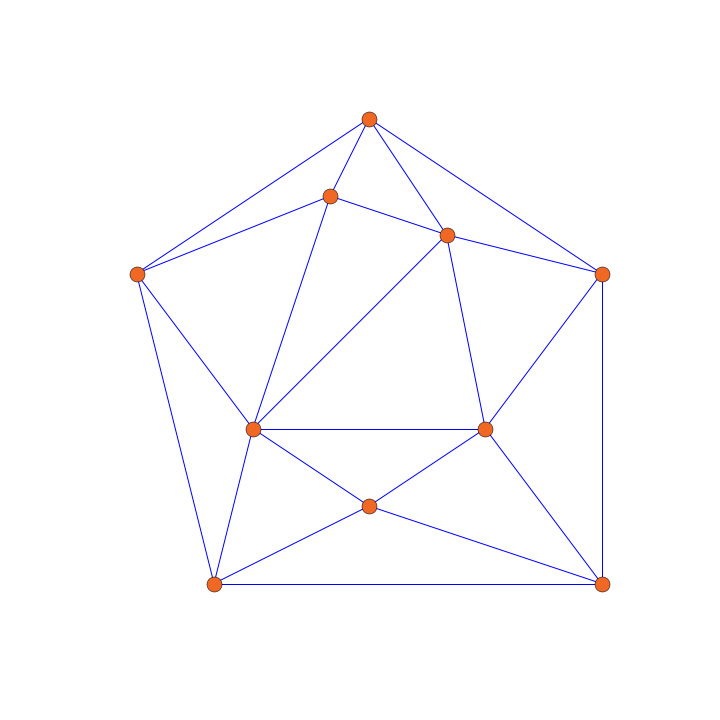
\includegraphics[width=0.8in, height=0.8in]{figs/tris_5}
  \label{fig:tris_5}
  }
  \subfigure[]{
  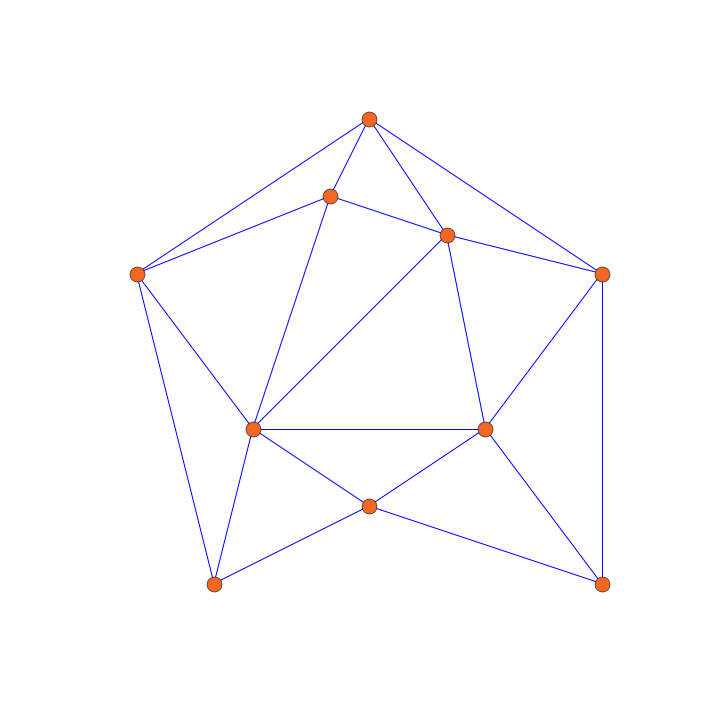
\includegraphics[width=0.8in, height=0.8in]{figs/tris_6}
  \label{fig:tris_6}
  }
  \subfigure[]{
  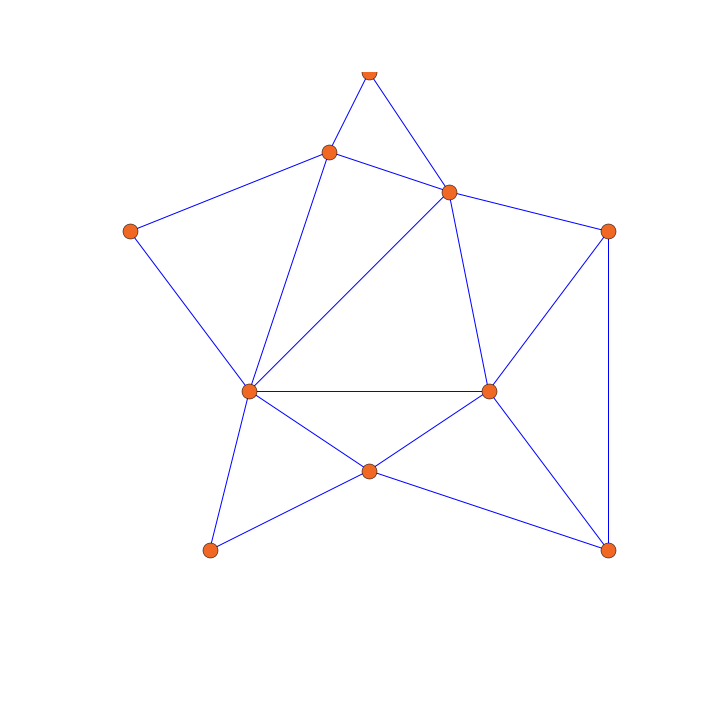
\includegraphics[width=0.8in, height=0.8in]{figs/tris_8}
  \label{fig:tris_8}
  }
  \subfigure[]{
  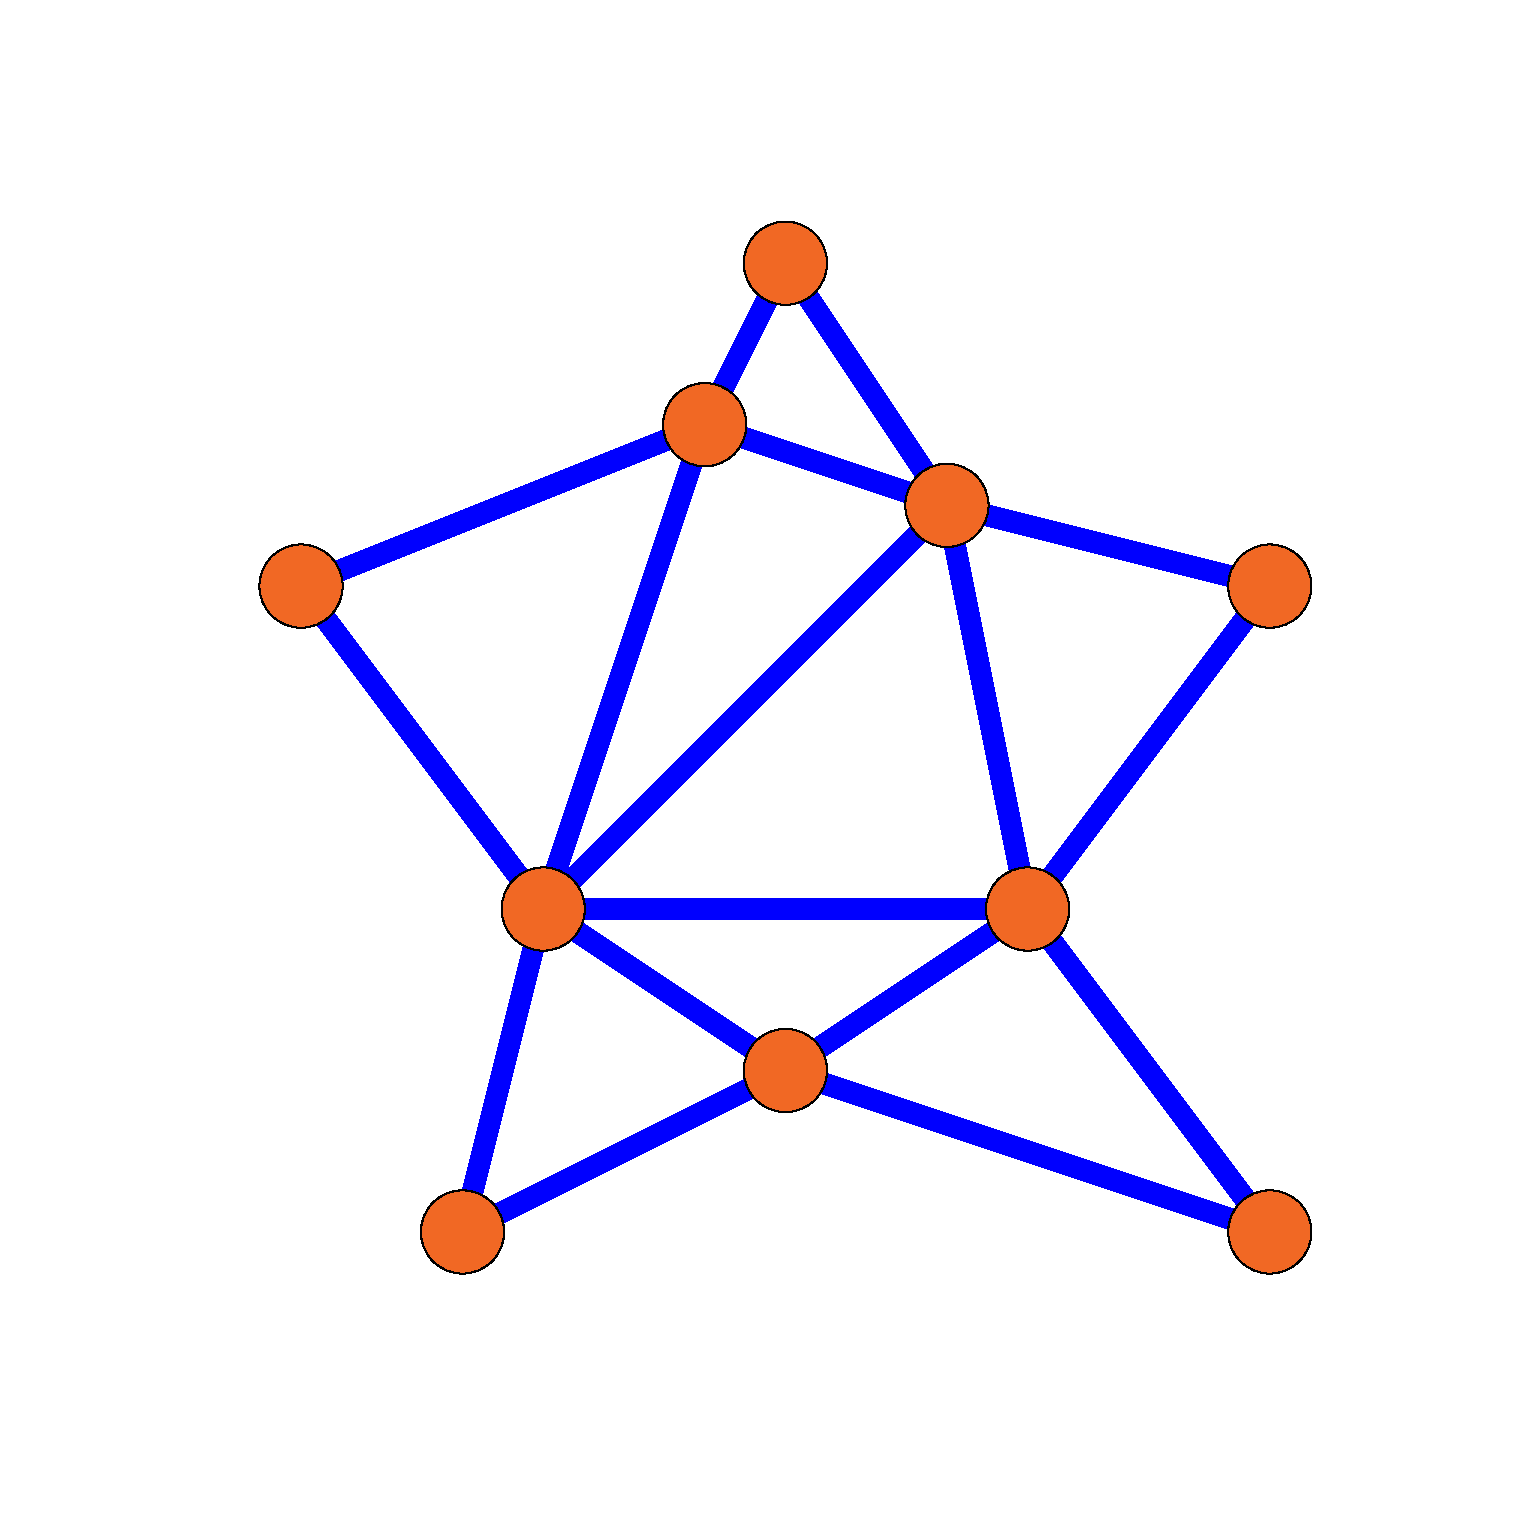
\includegraphics[width=0.8in, height=0.8in]{figs/tris_10}
  \label{fig:tris_10}
  }
  \subfigure[]{
  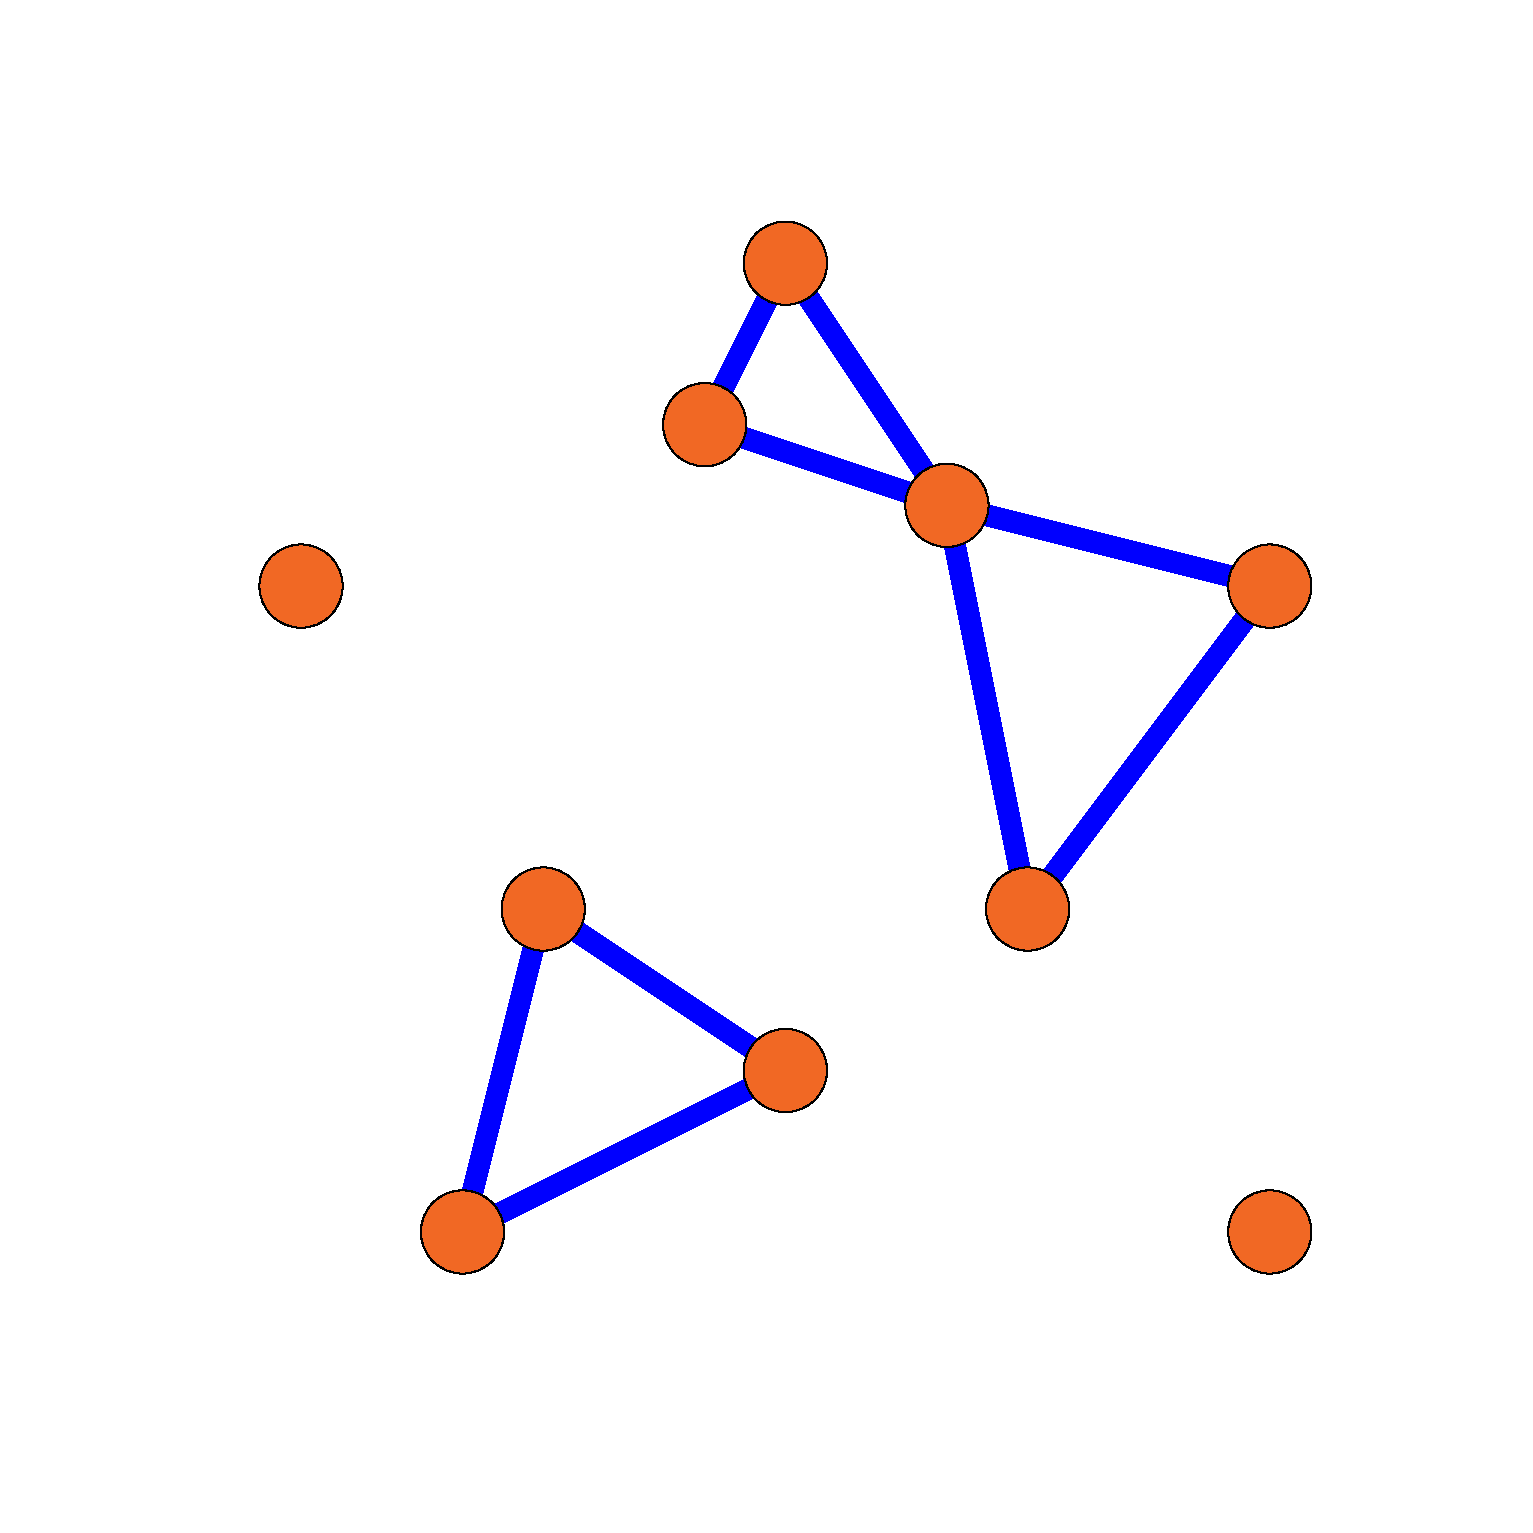
\includegraphics[width=0.8in, height=0.8in]{figs/tris_13}
  \label{fig:tris_13}
  }
  \caption{Simple example showing Delaunay triangulation and $\alpha$-shape calculation. The red circles are the point set.~\ref{fig:tris_5}-~\ref{fig:tris_13} show the Delaunay triangles that make up the $alpha$-shape for decreasing values of $\alpha$.~\ref{fig:tris_5} at $\alpha=\infty$ is equivalent to the Delaunay triangulation. As $\alpha$ decreases, triangles are removed that have a circumcircle with radius greater than $\alpha$. The $\alpha$-shape is the union of all triangles.}
  \label{fig:star}
\end{figure}

The lung shape is approximately convex along the pleural surface, so the convex hull of the initial mask gives a good estimate of the boundary for this surface, even in presence of large chest wall tumors. However, the mediastinum and diaphragm regions are not convex so the convex hull oversegments these regions. $\alpha$-shapes allow us to elegantly obtain a family of shapes that smoothly interpolates between the convex hull and initial mask to represent the lung shape. 


As the $\alpha$-shape is defined on a point set, rather than an image, first we obtain a set of points $p \in P$ representing the initial mask. We could use the physical locations of all image voxels in the mask as our point set, however for time efficiency we chose to only take a sample of these voxels. We performed image erosion and subtraction operations to generate a set of concentric contours of the initial mask and used these voxel locations for $P$. To ensure all of the initial mask is included in the $\alpha$-shape, the separation between concentric contours needs to be small enough such that the d-simplices formed between contours have a circumradius smaller than $\alpha$. 


There is a trade off between over segmentation and under segmentation when choosing $\alpha$. When $\alpha$ is too large, the mediastinum is over segmented, however decreasing $\alpha$ too much can remove tumors (Figure~\ref{fig:alphashapes}).  We experimented with different values of $\alpha$ to obtain lung shapes the included tumor regions and minimized oversegmentation near the diaphragm and mediastinum. The diaphragm is easily removed due to the broad concave structure, however the mediastinum has many very small concavities resulting in minor oversegmentation that cannot be removed without removing the tumor. We empirically determined $ \alpha=25 $ to give good results for all subjects in this study. Prior to the next step, we performed Laplacian smoothing~\cite{herrmann1976} on the alpha shape surface to remove sharp edges. 

%
% http://texblog.org/2007/08/28/placing-figurestables-side-by-side-subfigure/
%
\begin{figure}[ht!]
  \centering
  \subfigure[CT]{
  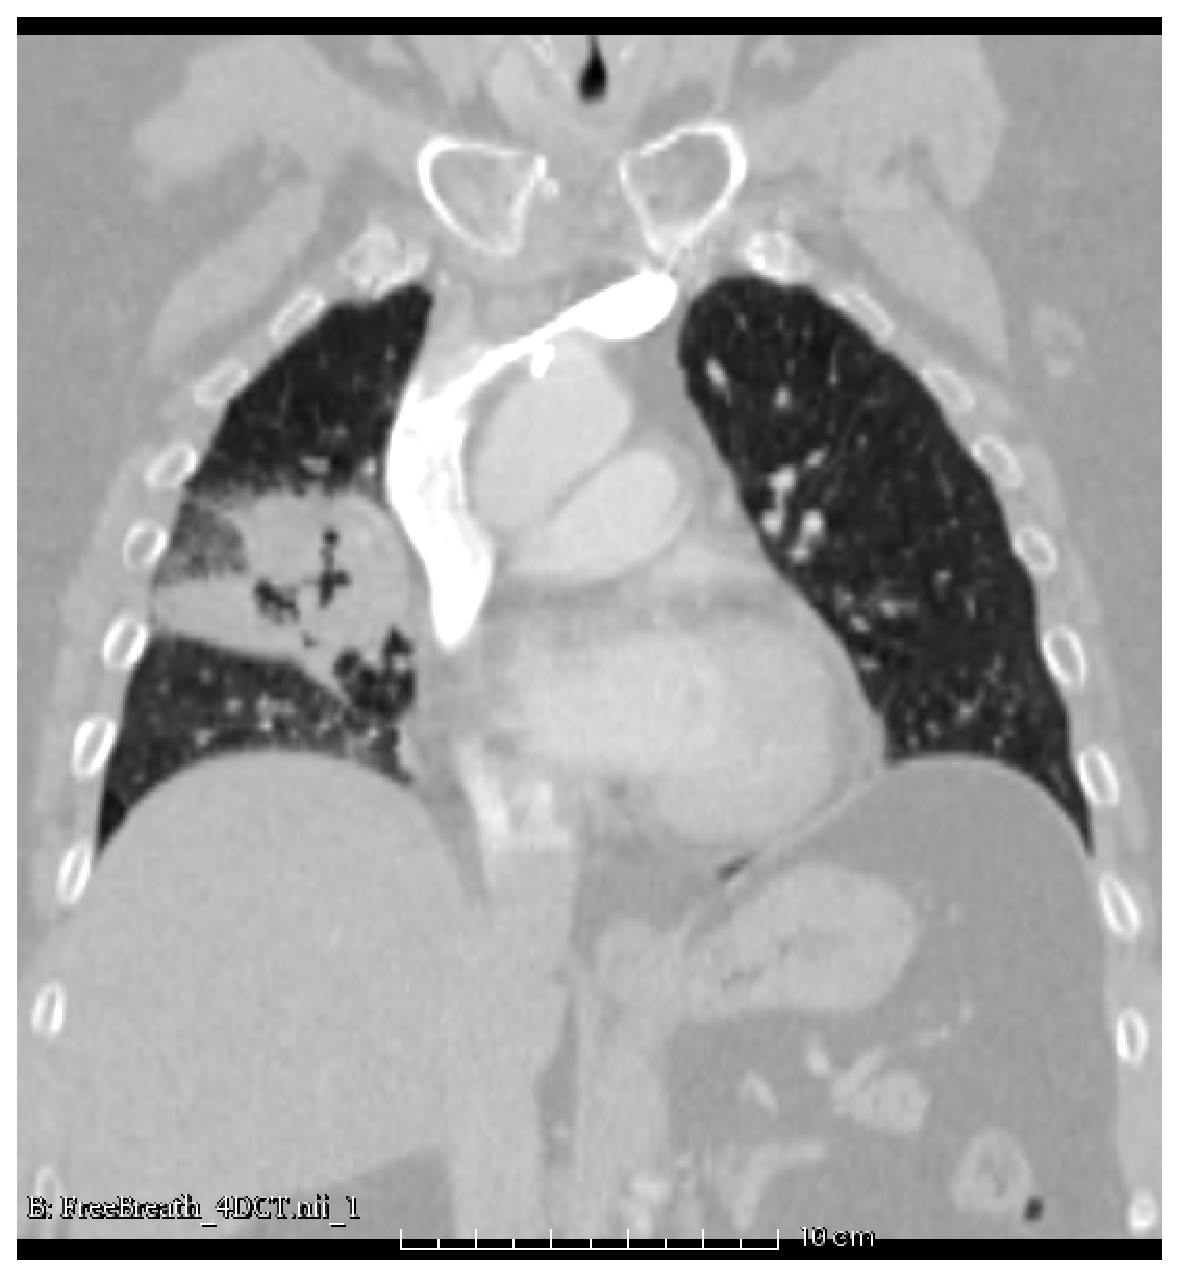
\includegraphics[trim={5 160 340 110},clip,width=1.0in, height=1.4in]{figs/ct}
  \label{fig:tris_CT}
  }
  \subfigure[Initial Mask]{
  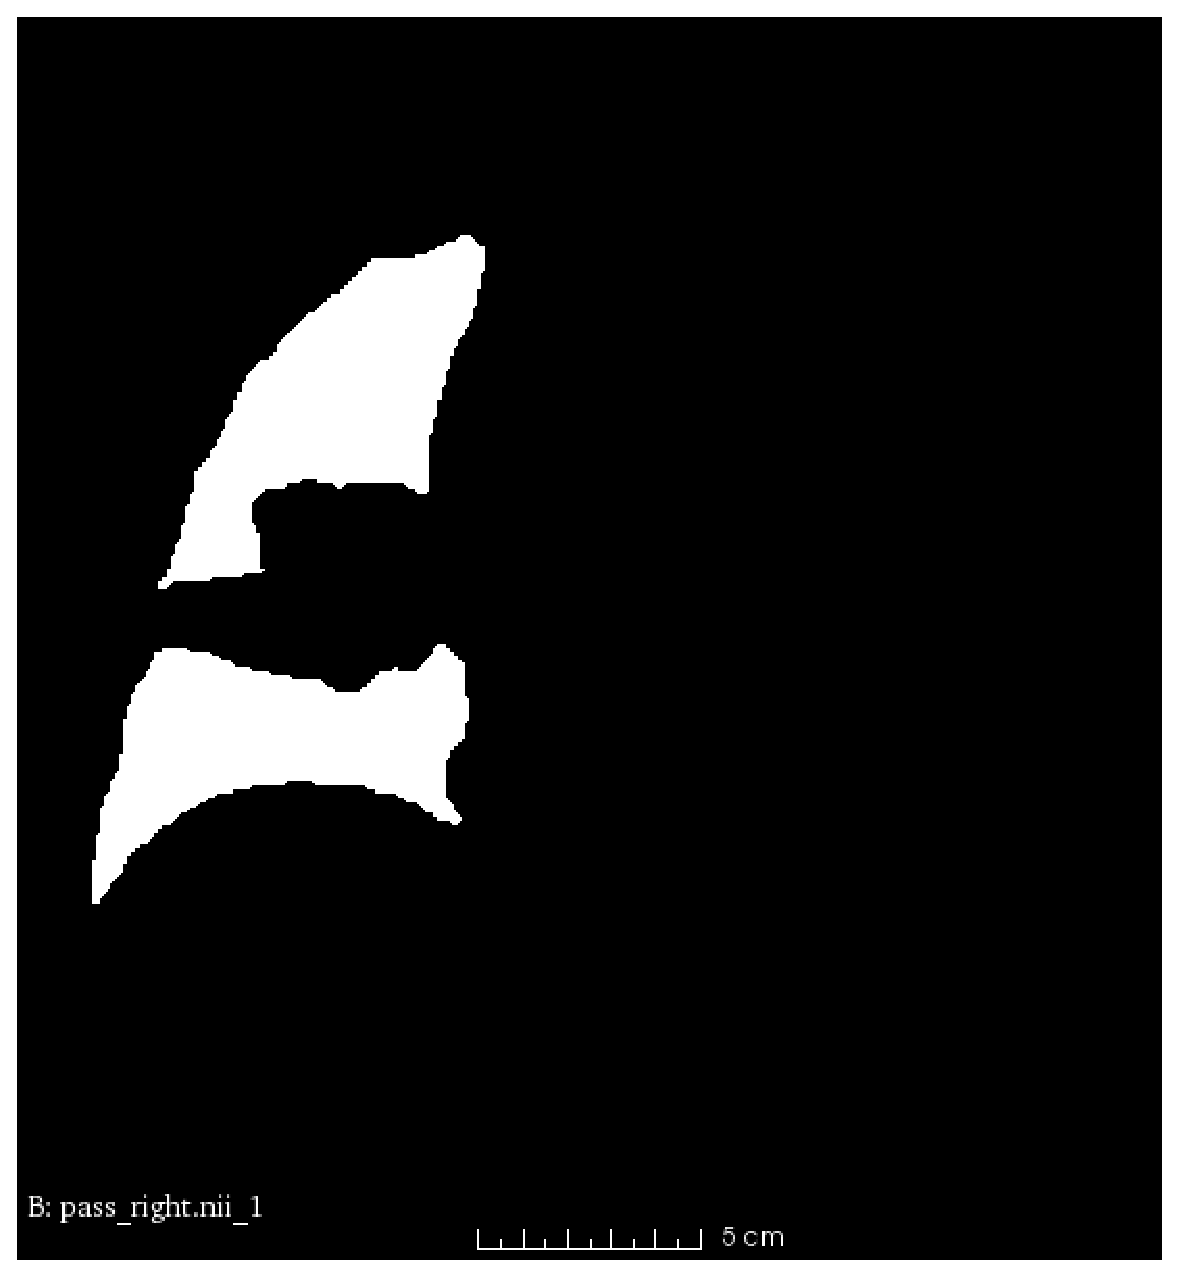
\includegraphics[trim={5 150 300 100},clip,width=1.0in, height=1.4in]{figs/pass}
  \label{fig:tris_Mask}
  }
  \subfigure[Point Set]{
  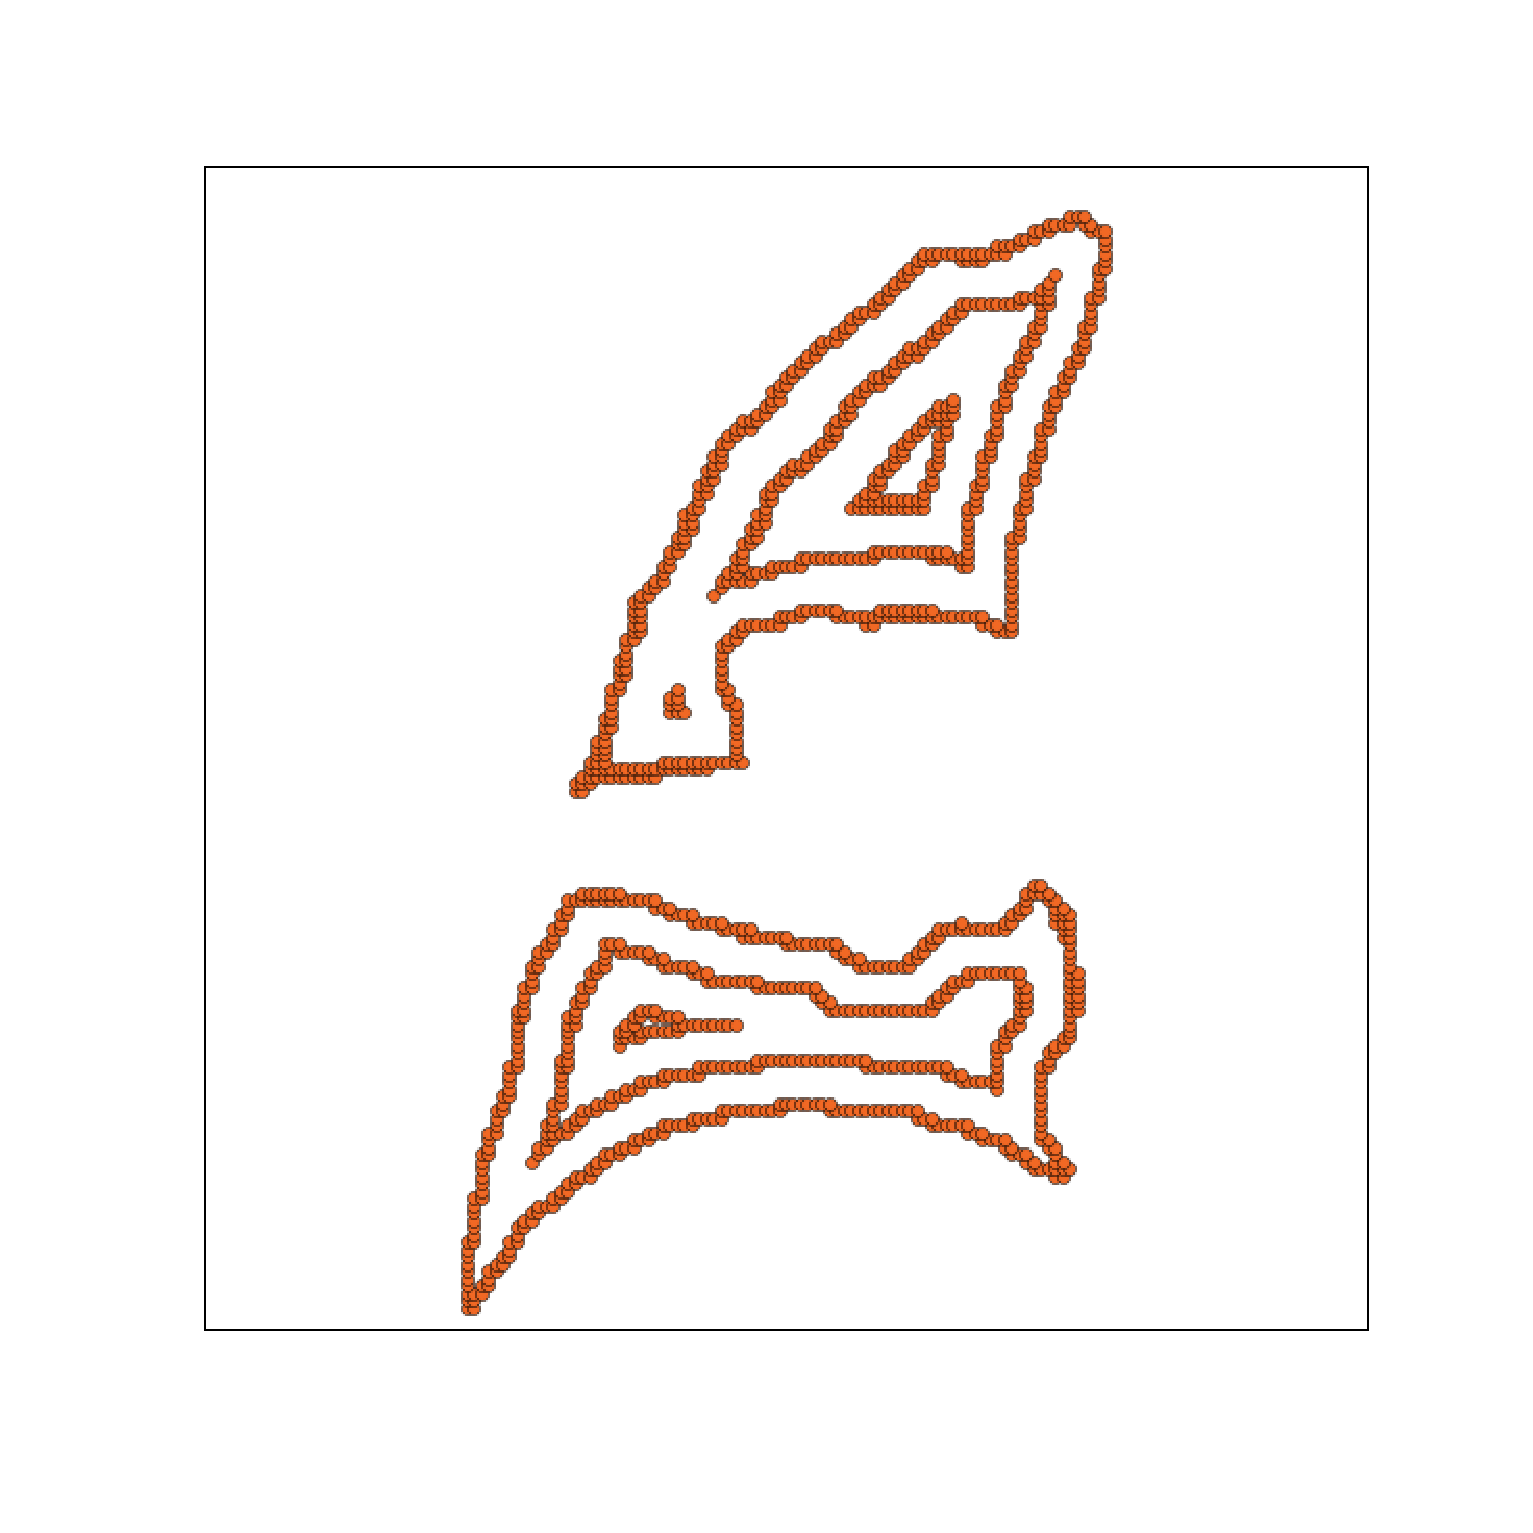
\includegraphics[trim={150 100 150 100},clip,width=1.0in]{figs/points}
  \label{fig:tris_points}
  }
  \subfigure[$\alpha = 200$]{
  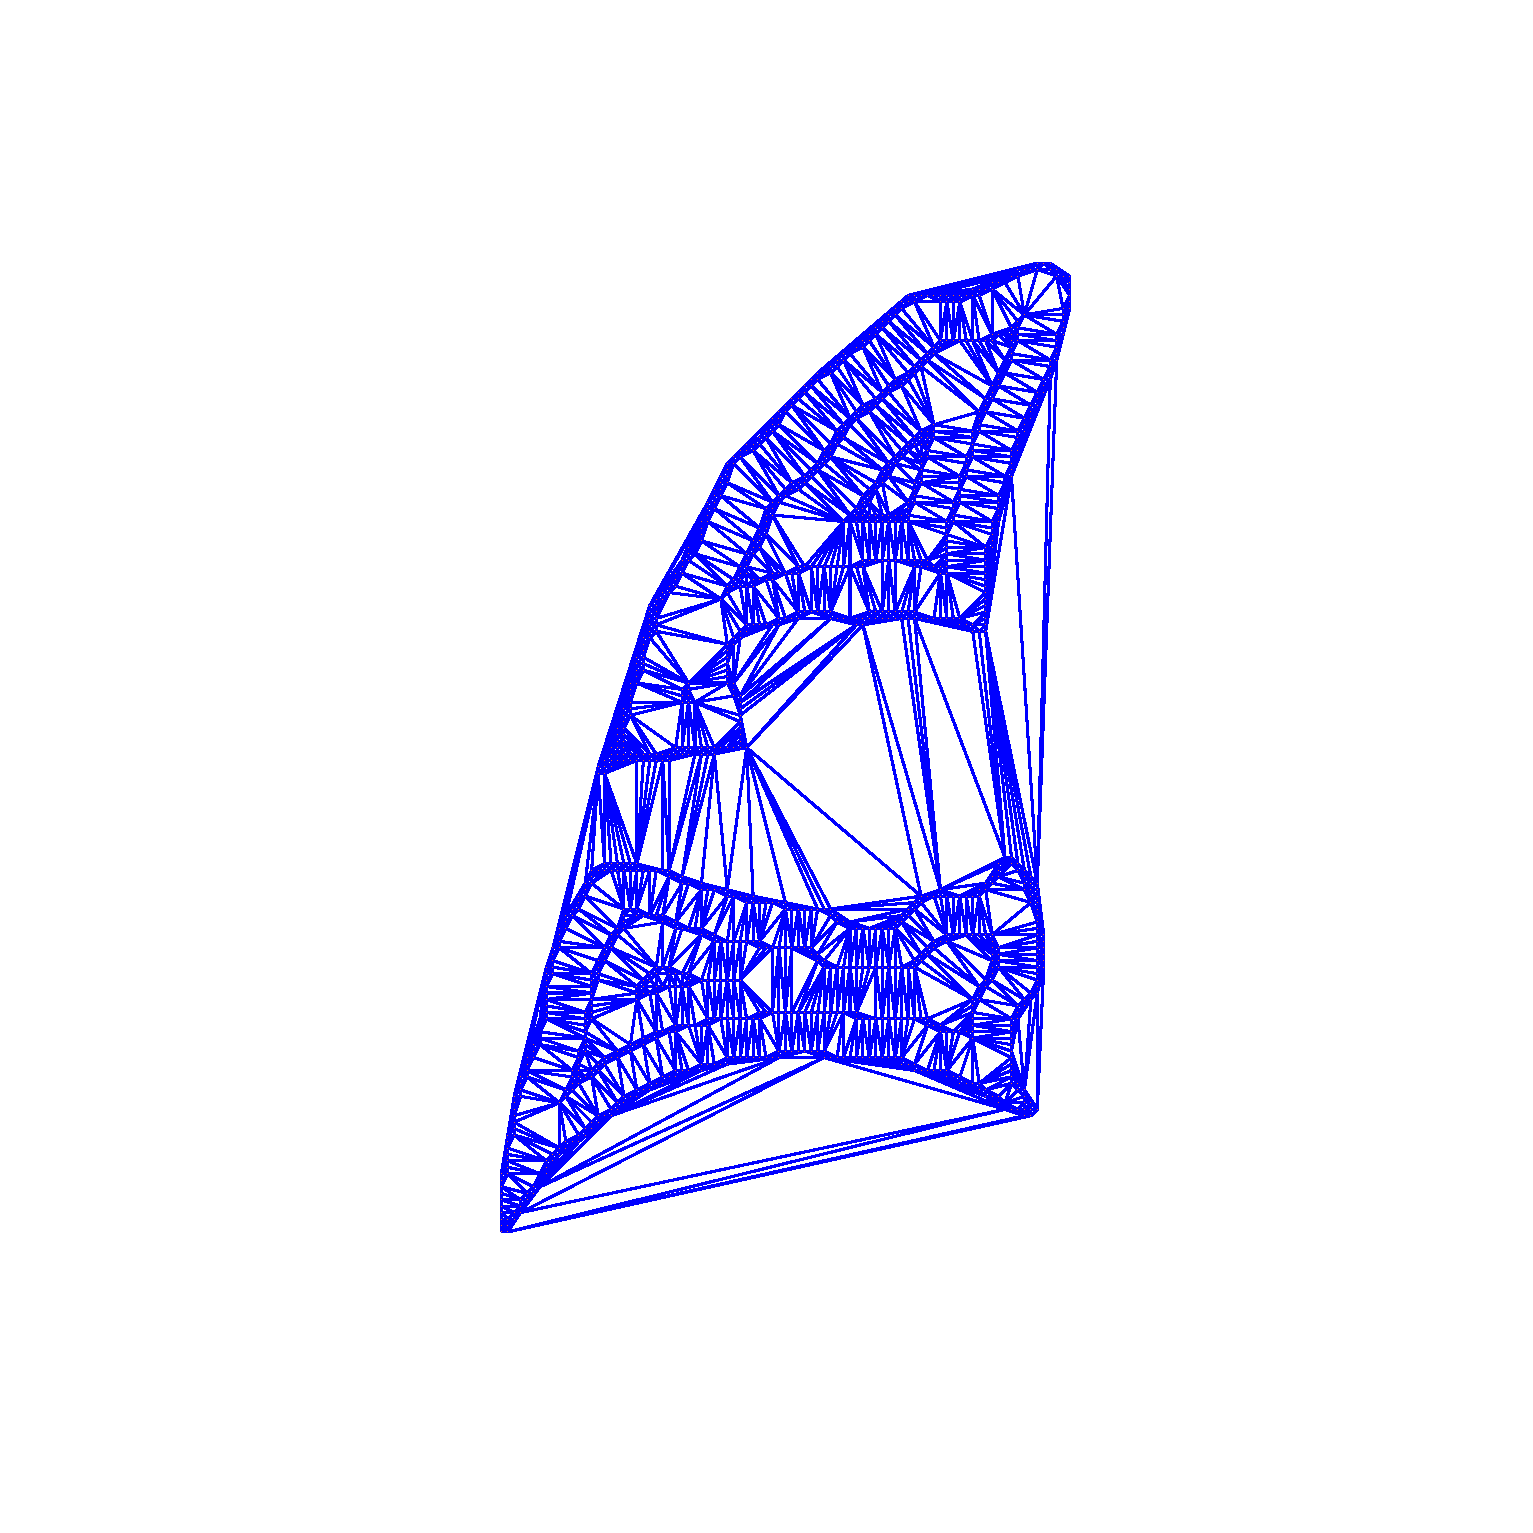
\includegraphics[trim={150 100 150 100},clip,width=1.0in]{figs/tris_200}
  \label{fig:tris_alpha_200}
  }
  \subfigure[$\alpha = 66$]{
  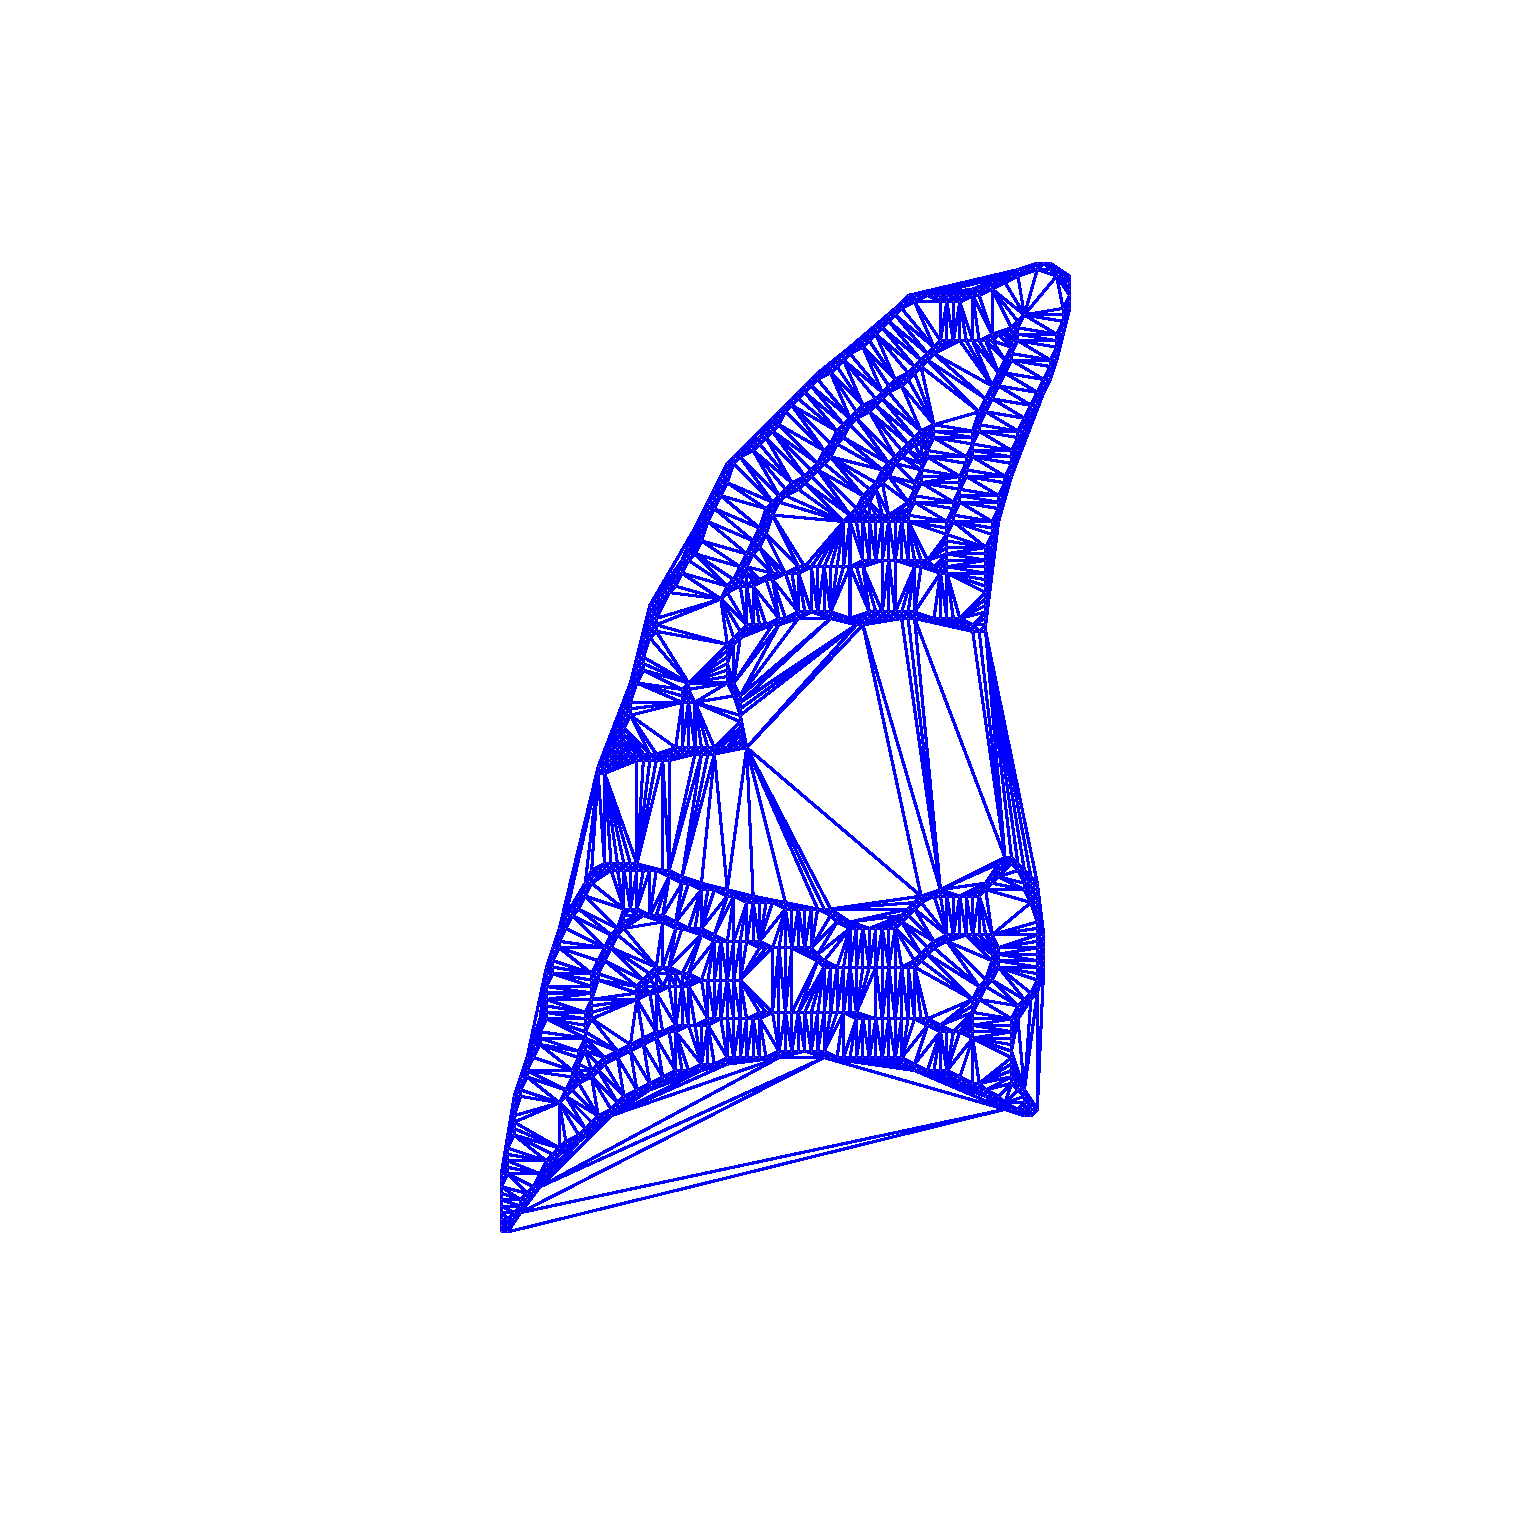
\includegraphics[trim={150 100 150 100},clip,width=1.0in]{figs/tris_66}
  \label{fig:tris_alpha_66}
  }
  \subfigure[$\alpha = 50$]{
  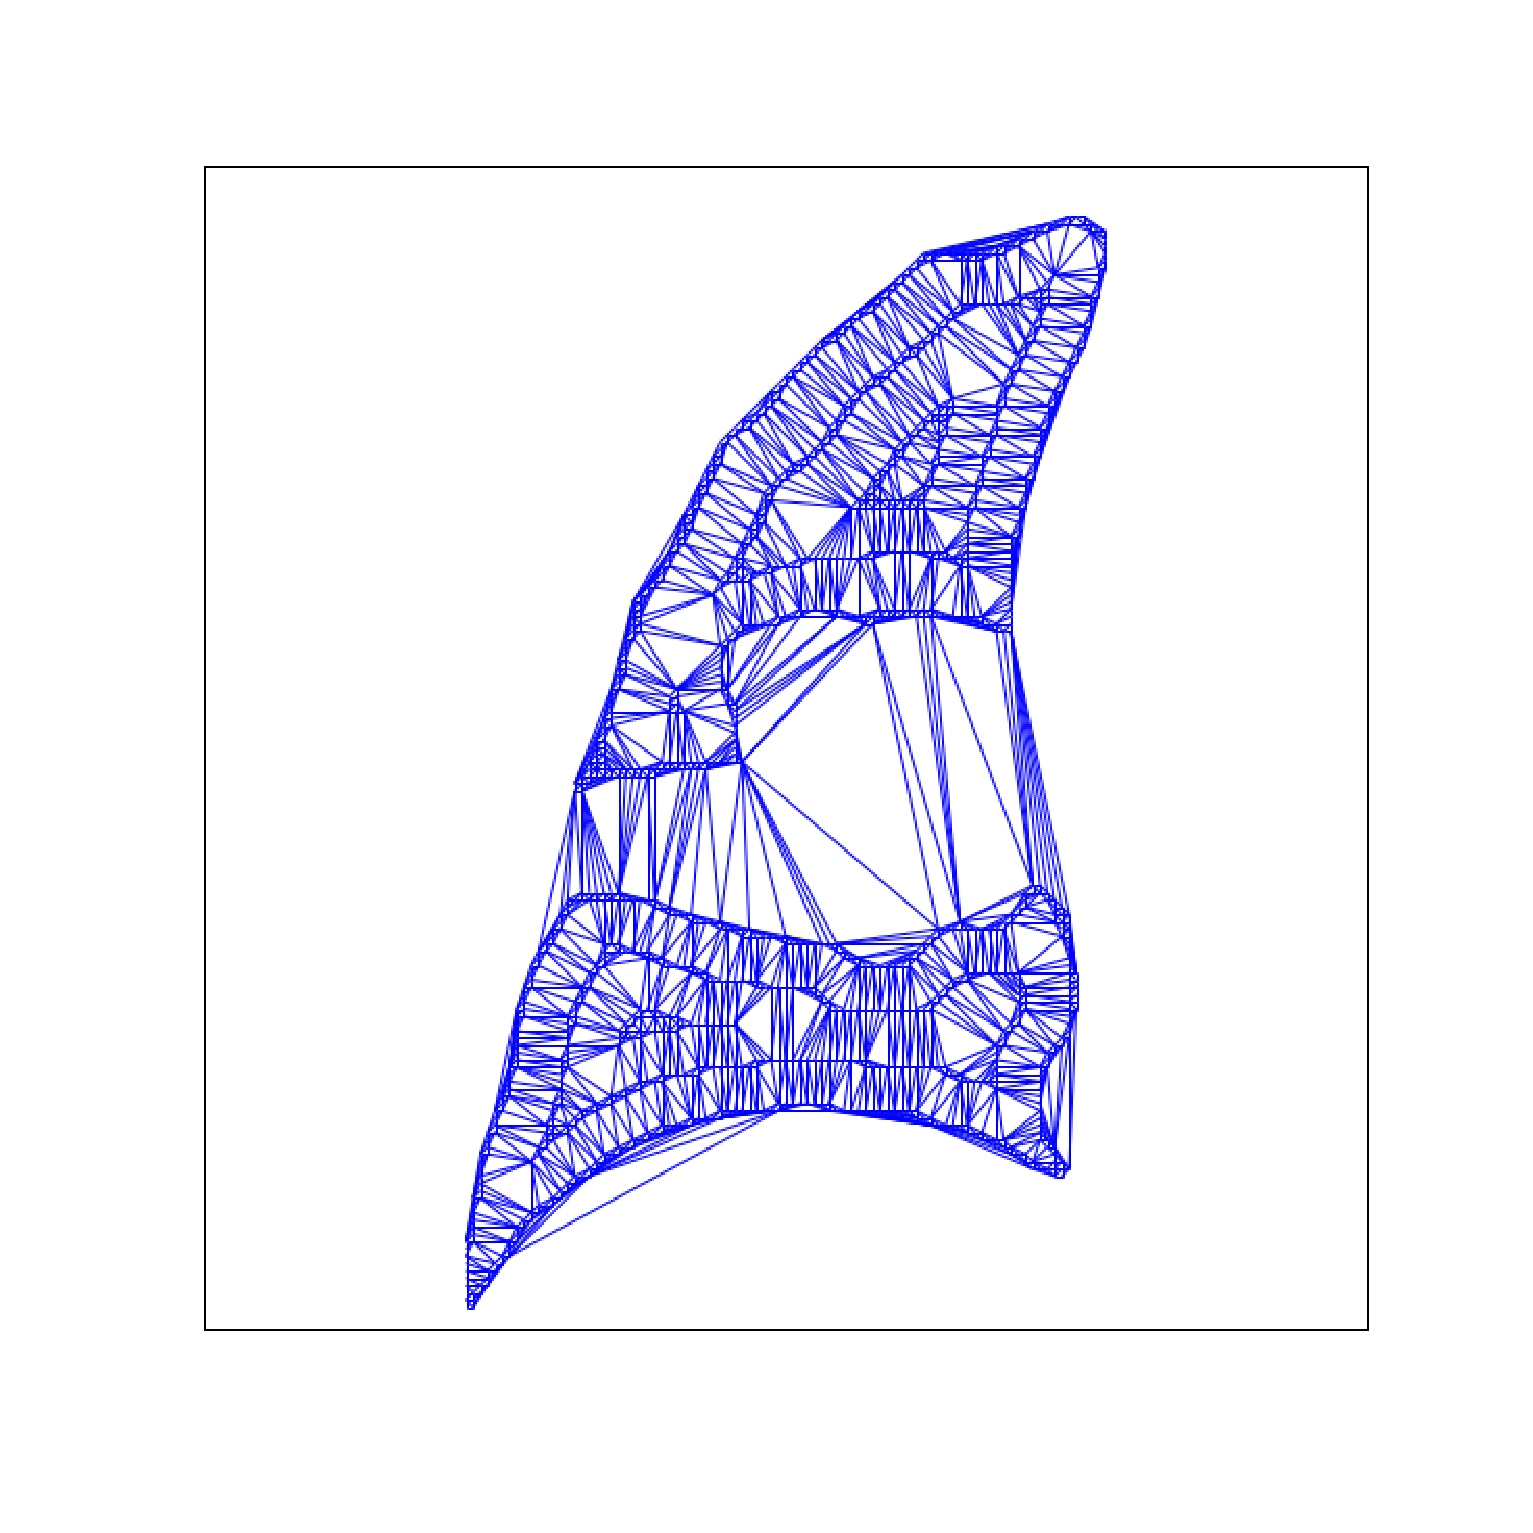
\includegraphics[trim={150 100 150 100},clip,width=1.0in]{figs/tris_50}
  \label{fig:tris_alpha_50}
  }
  \subfigure[$\alpha = 33$]{
  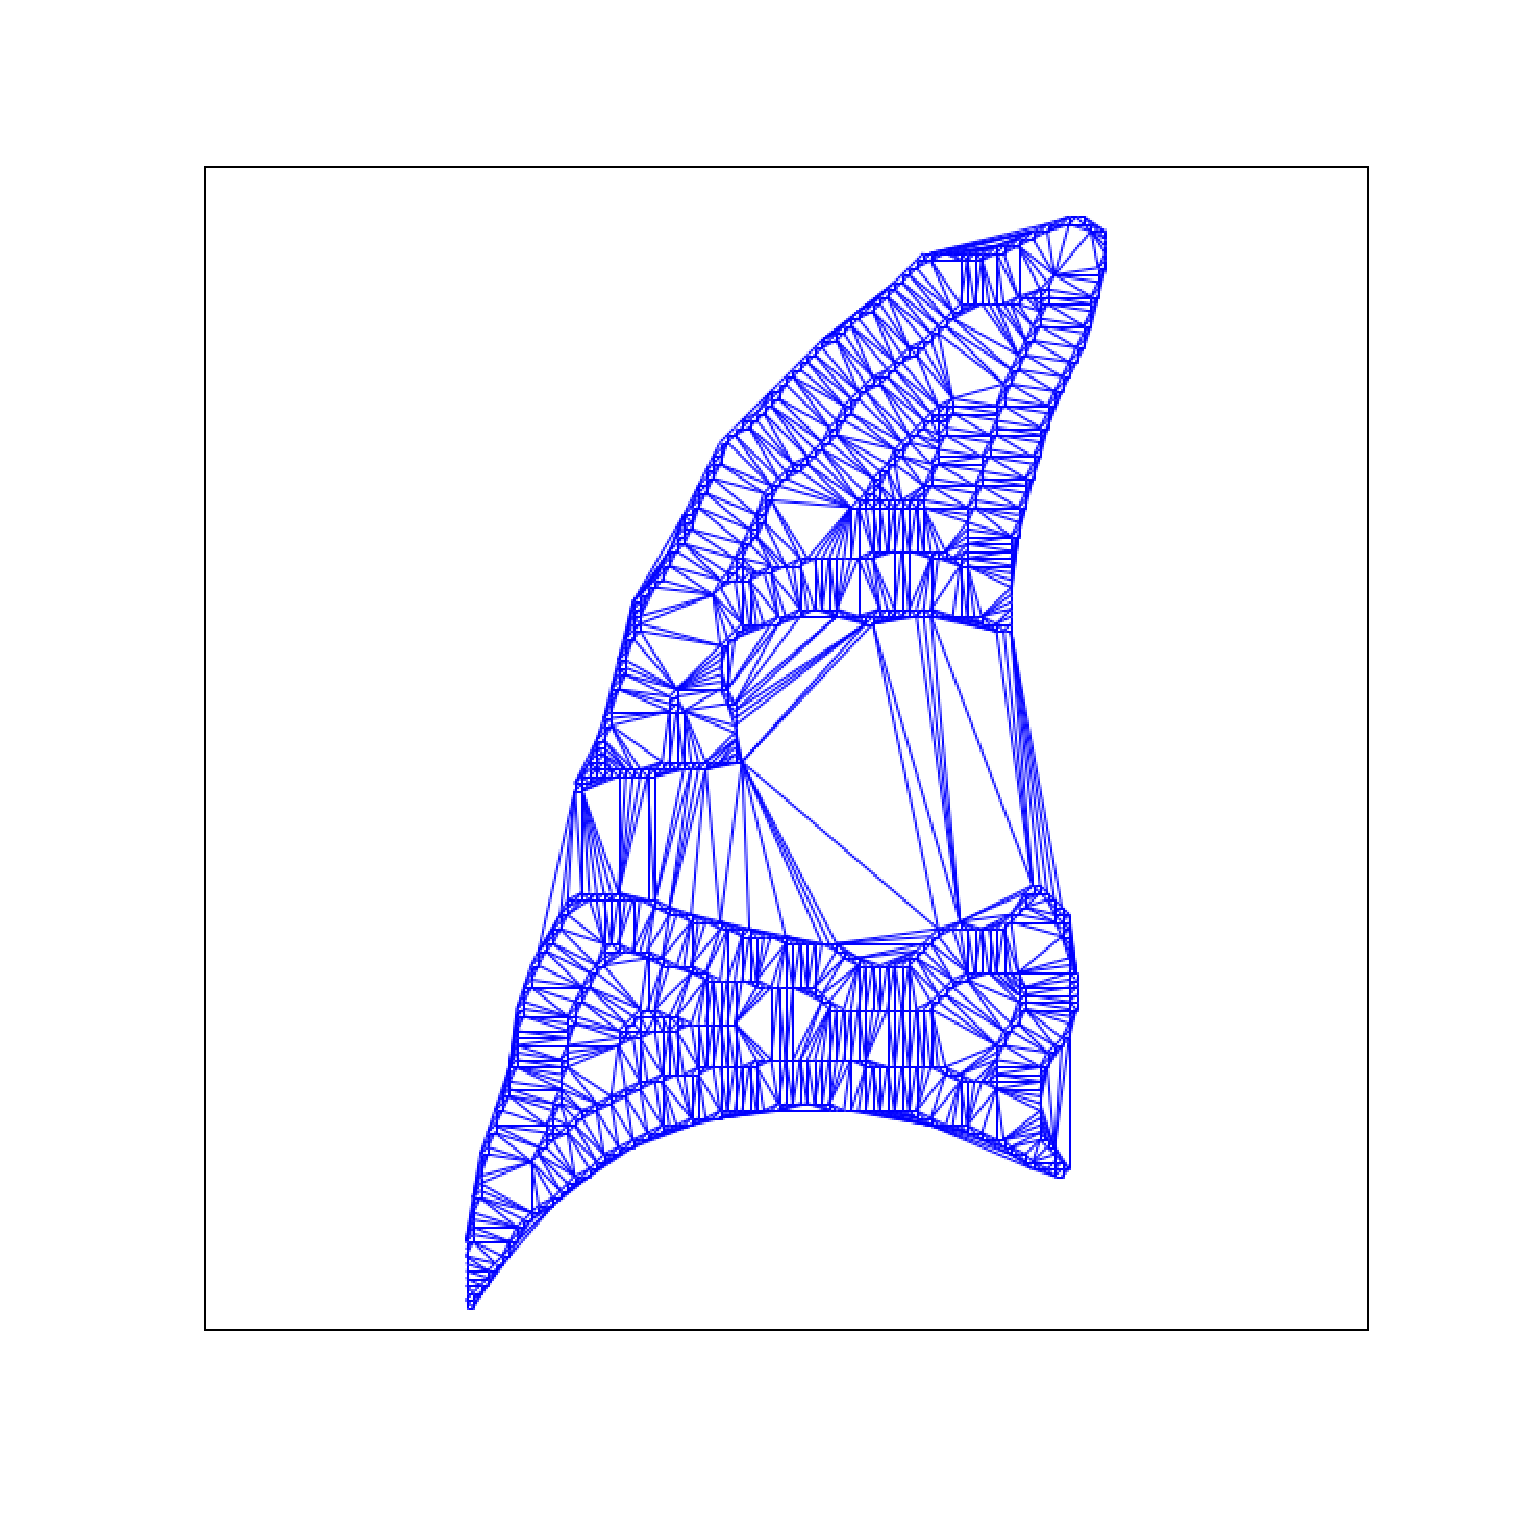
\includegraphics[trim={150 100 150 100},clip,width=1.0in]{figs/tris_33}
  \label{fig:tris_alpha_33}
  }
  \subfigure[$\alpha = 15$]{
  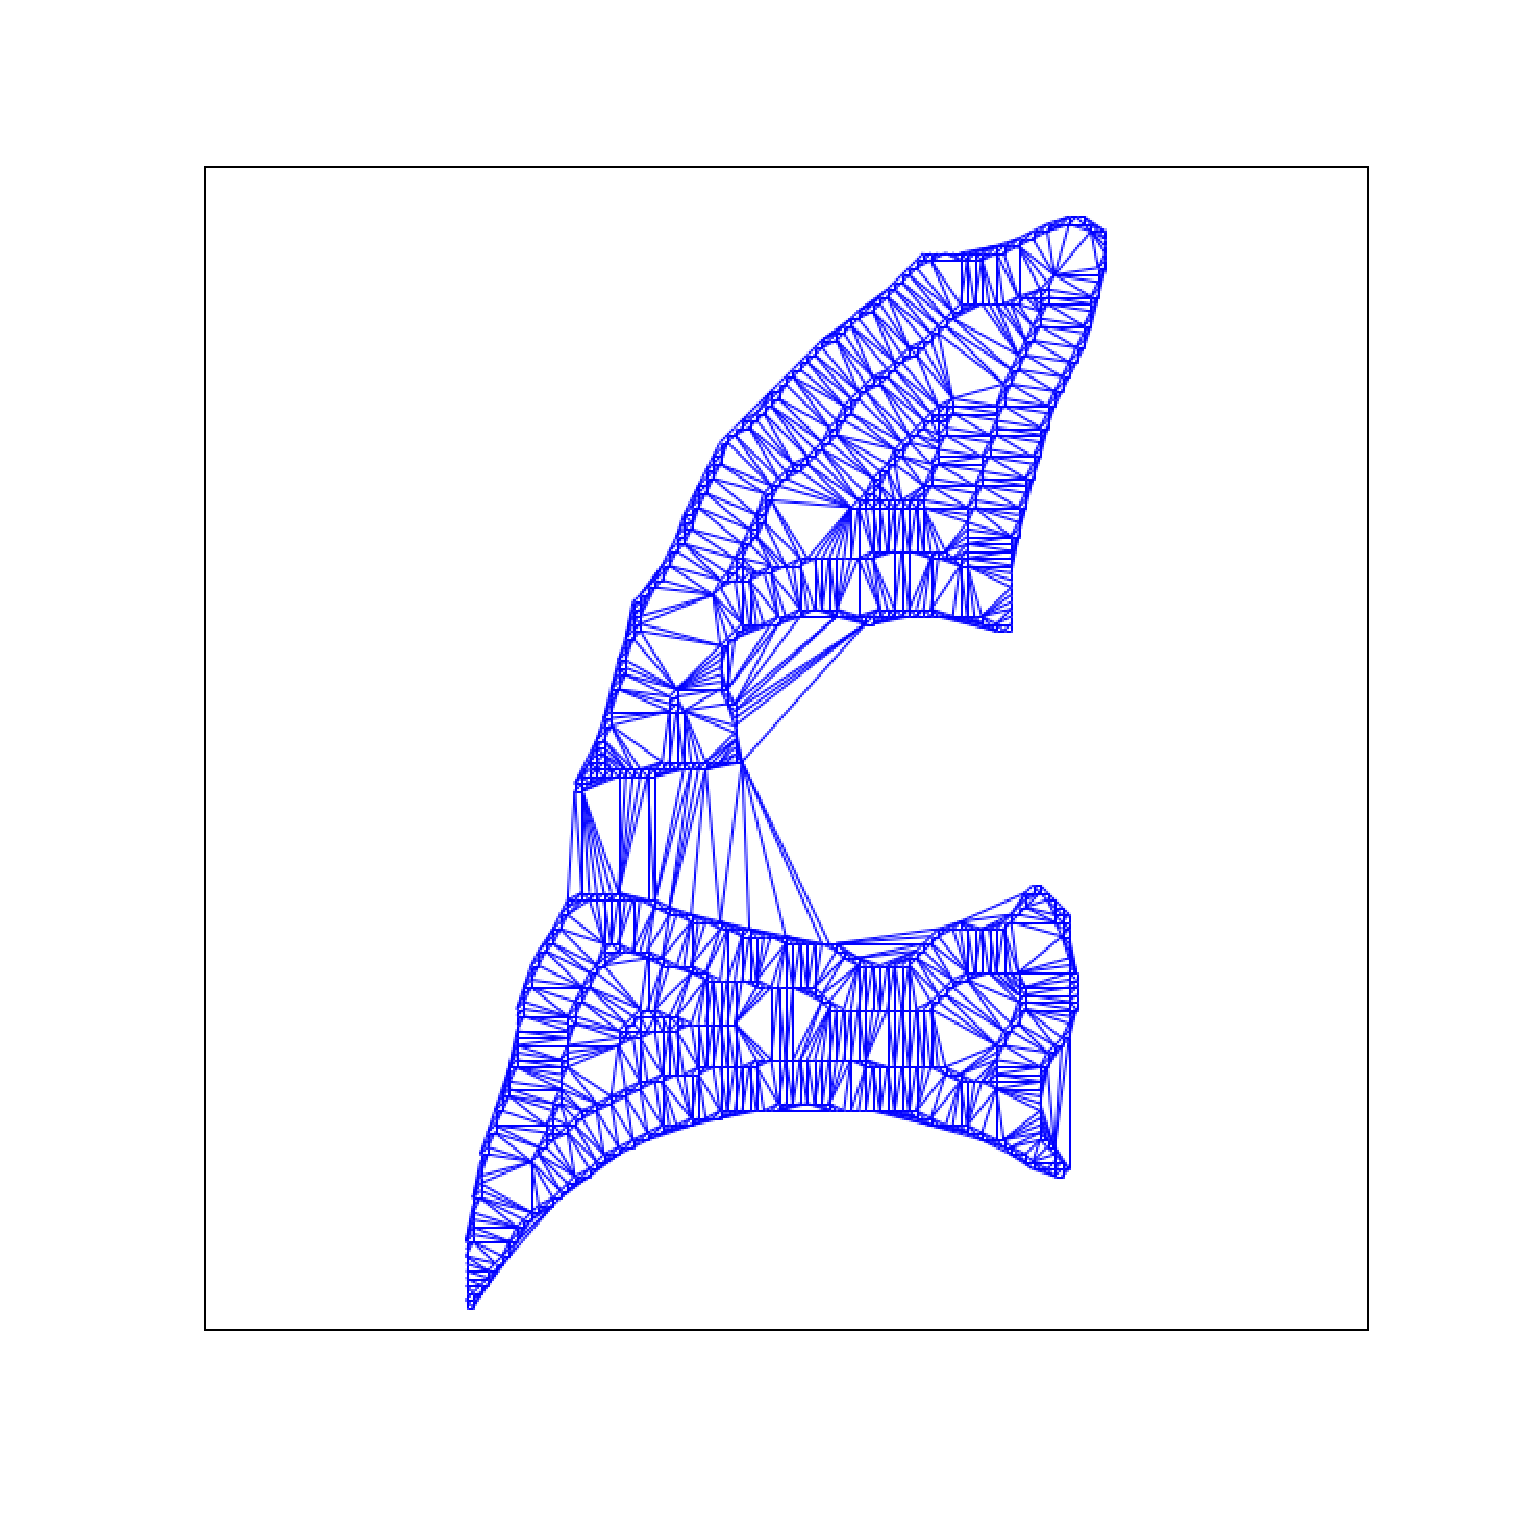
\includegraphics[trim={150 100 150 100},clip,width=1.0in]{figs/tris_15}
  \label{fig:tris_alpha_15}
  }
  \caption{~\ref{fig:tris_CT} CT image showing large radiodense tumor in right lung, ~\ref{fig:tris_Mask} initial mask produced by thresholding, ~\ref{fig:tris_points} point set used to represent initial mask,~\ref{fig:tris_alpha_200}-~\ref{fig:tris_alpha_15} Delaunay triangles that form the alpha shape for decreasing alpha values. Note: this is a 2D example for illustrative purposes; the actual method is performed in 3D with tetrahedrons instead of triangles. }
  \label{fig:tris}
\end{figure}


\begin{figure}[t]
  \centering
    \subfigure[$\alpha = 200$]{
    \includegraphics[trim={100 5 100 5},clip, width=1.3in]{figs/alpha_inf} 
    \label{fig:img_alpha200}
    }
    \subfigure[$\alpha = 25$]{
    \includegraphics[trim={100 5 100 5},clip, width=1.3in]{figs/alpha_seg}
    \label{fig:img_alpha25}
    }
    \subfigure[$\alpha = 9$]{
    \includegraphics[trim={100 5 100 5},clip, width=1.3in]{figs/alpha_zero} 
    \label{fig:img_alpha9}
    }
  \caption{Alpha shape of initial mask for different values of $\alpha$.~\ref{fig:img_alpha200} is approximately equal to the convex hull of the initial mask,~\ref{fig:img_alpha9} is approximately equal to the initial mask.}
  \label{fig:alphashapes}
\end{figure}
%
\subsection{Graph Search}
%
To reduce minor mediastinum oversegmentation resulting from small concavities, we use a graph search framework to find the optimal lung surface. The method will only briefly be described here; see~\cite{li2006} for a detailed description of the method. 

The graph search method requires a shape prior, here we use the alpha shape from the previous step as the shape prior. A graph $G(E,V)$ consisting of node set $V$ and edge set $E$ is built in a margin around the shape prior. The nodes have an associated cost reflecting the unlikeliness that it belongs to the lung surface. We use the inverse gradient of the CT image for the cost, as the lung surface has a high image gradient. Edges are used to enforce smoothness constraints, or how much the topology of the resulting segmentation can deviate from the shape prior. The globally optimal surface is obtained by using a maximum flow algorithm on a closely derived graph. 

As a final step we performed a logical OR operation between the graph search result and the initial mask. This adds back in sharp edges, such as those at the costophrenic angle, that are lost when the smoothing is performed.
 

%
\section{Data Sets and Experimental Setup}
%
In this study we used breath-hold thoracic CT scans from twelve lung cancer subjects about to undergo radiation therapy. All scans were gathered under a protocol approved by the 
XXXXXXXXXXX YYYYYYY 
%University of Iowa 
Institutional Review Board 
%(IRB 200905703). 
(IRB ZZZZZZZZZ).
All images were resampled from $0.98\times{}0.98\times{}2$ mm$^3$ to obtain $1\times{}1\times{}1$ mm$^3$ isotropic voxels. We chose 11 subjects that had a large lung tumor in either left or right lung, and 1 subject with no lung tumors.

Our method was evaluated by comparing to manual segmentations generated by a radiation therapy physicist using the MimVista 6.4.7 software (MIM Software, Cleveland, OH) following a protocol similar to that used for radiation therapy planning. The DICE coefficient was used for a metric of volume overlap, and the average unsigned symmetric surface distance was used to measure the distance between the lung boundaries. The analysis was performed on both the left and right lungs of all subjects. Additionally, we compared the results of lungs with and without tumors.


The proposed method was implemented using the jupyter notebook~\cite{PER-GRA:2007} rapid prototyping environment,  algorithms from ITK~\cite{johnson2015itk} python wrapped in SimpleITK~\cite{10.3389/fninf.2013.00045} in coordination with vtkDelaunay3D from VTK (www.vtk.org).


%
\section{Results}
%
Figure~\ref{fig:dist} shows the average unsigned surface distances for the initial mask and our final segmentation for both tumor and non-tumor groups. Figure~\ref{fig:resultseg} shows the result at each step of the proposed method and the manual segmentation. 
\begin{figure}[ht!]
  \centering
    \subfigure[]{
    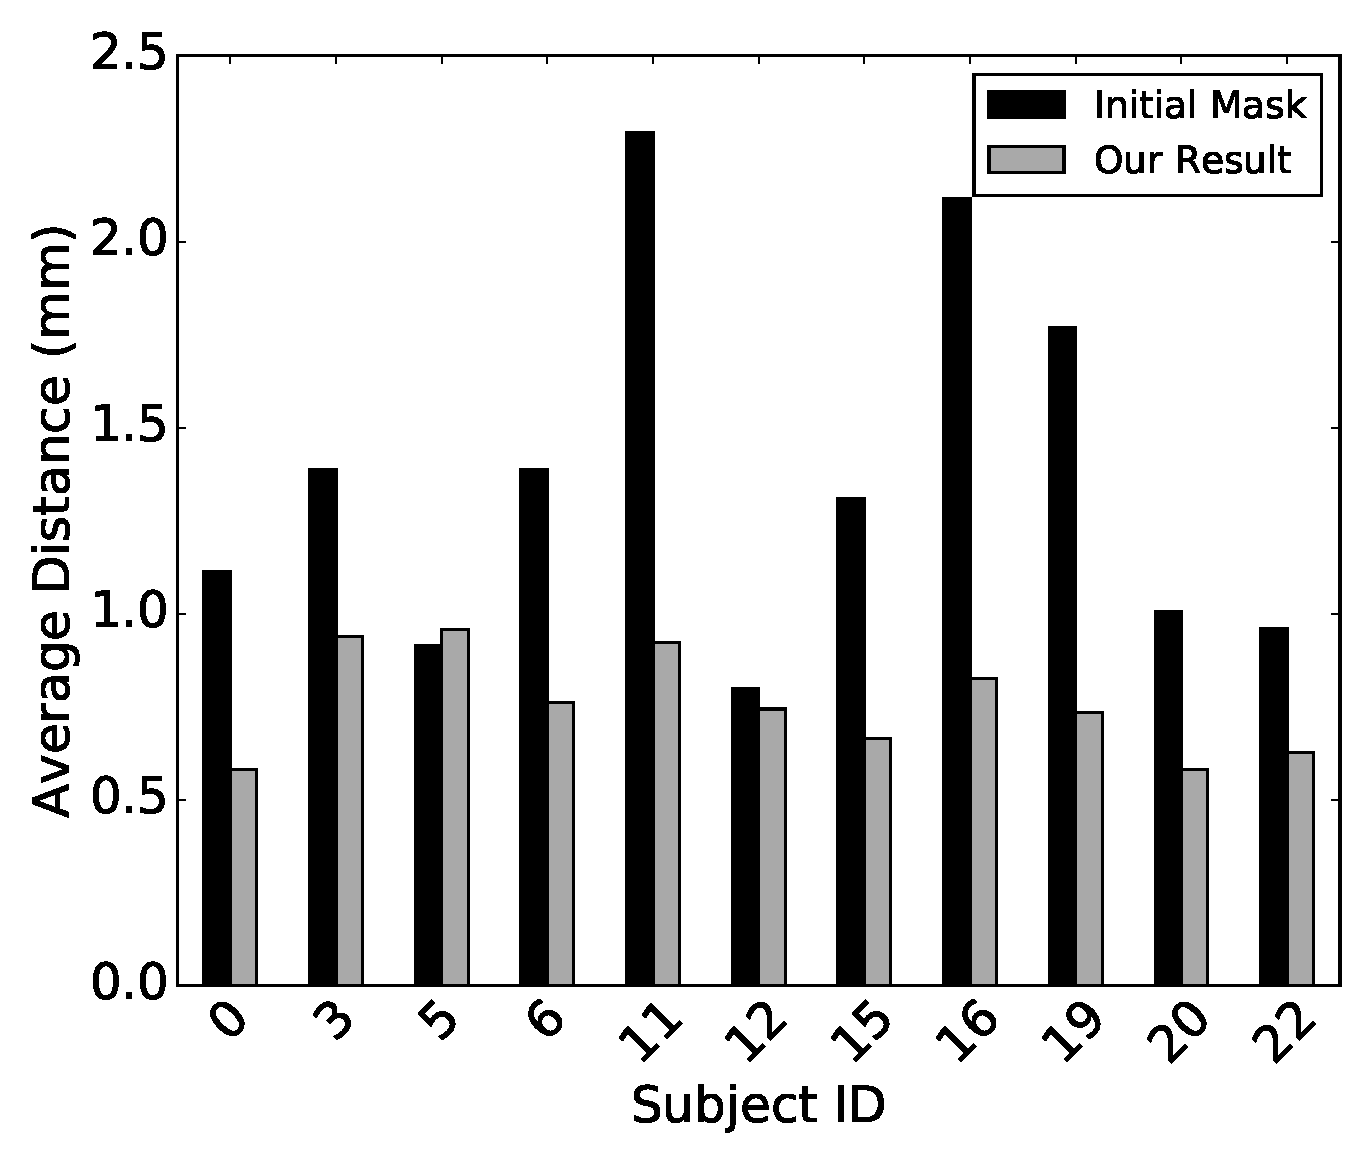
\includegraphics[width=2.2in]{figs/dist_tumor}
    \label{fig:dist_tumor}
    }
    \subfigure[]{
    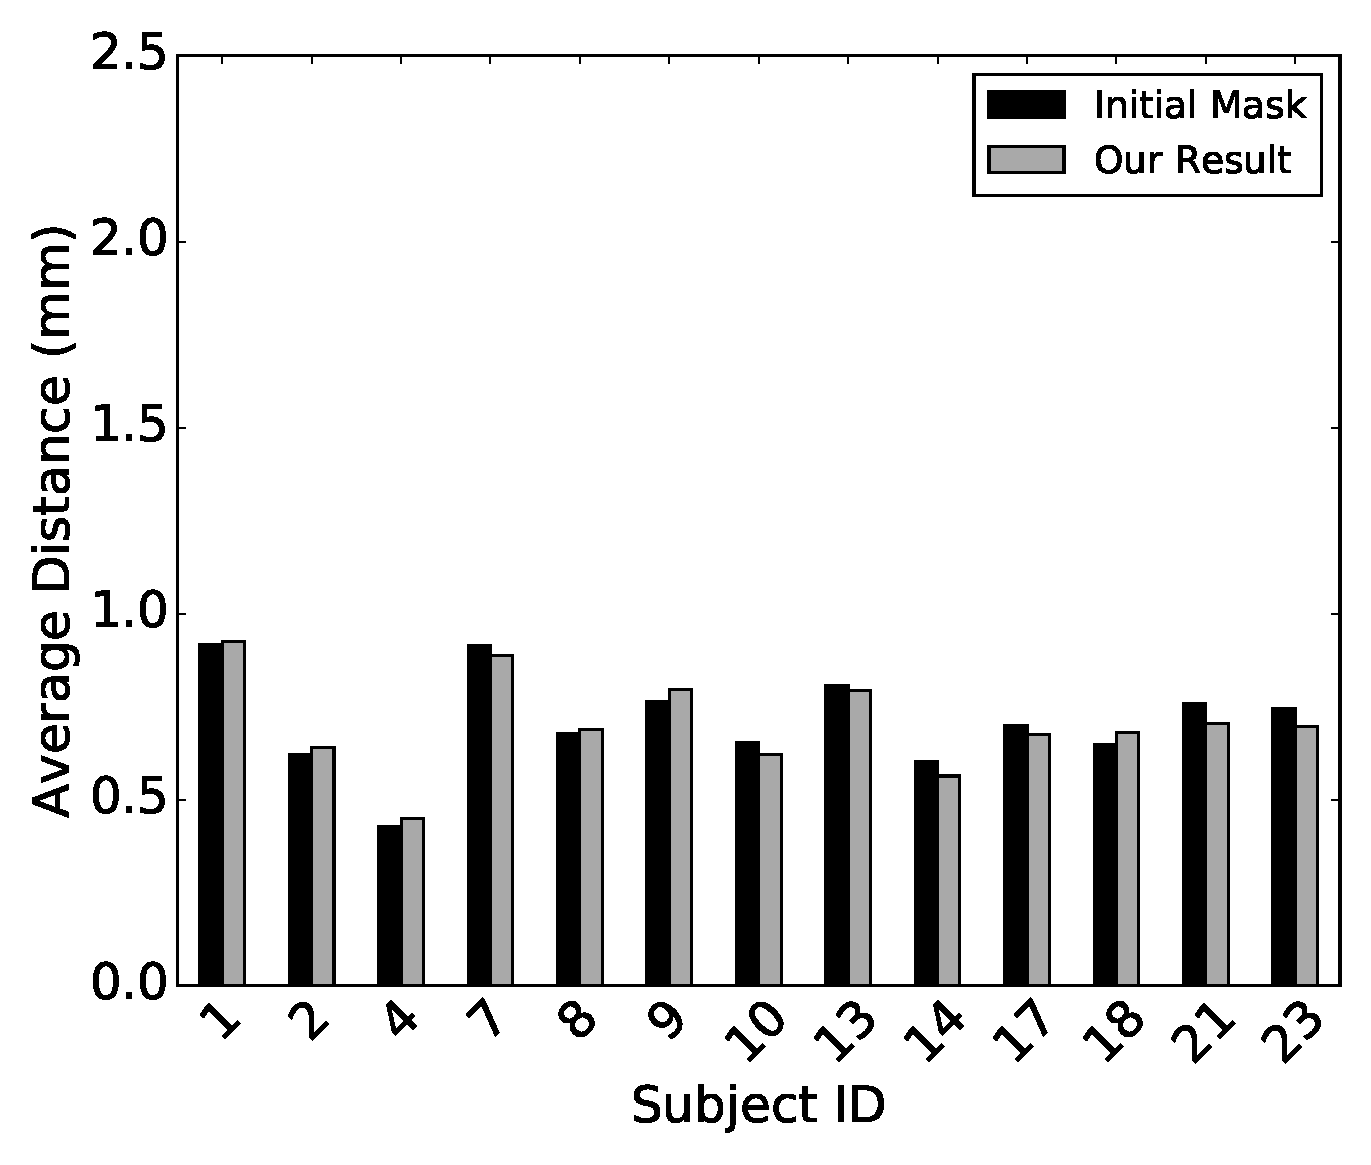
\includegraphics[width=2.2in]{figs/dist_nontumor}
    \label{fig:dist_nontumor}
    }
  \caption{Average unsigned surface distances for both the initial mask and our final result compared to the manual segmentation.~\ref{fig:dist_tumor} and~\ref{fig:dist_nontumor} show results for lungs with and without tumors, respectively.}
  \label{fig:dist}
\end{figure}

\begin{figure}[ht!]
  \centering
    \subfigure{
    \includegraphics[width=1.08in]{figs/PFS-002_ct}
    \label{fig:PFS-002_ct}
    }
    \subfigure{
    \includegraphics[width=1.08in]{figs/PFS-020_ct}
    \label{fig:PFS-020_ct}
    }
    \subfigure{
    \includegraphics[width=1.08in]{figs/PFS-031_ct}
    \label{fig:PFS-031_ct}
    }
    \subfigure{
    \includegraphics[width=1.08in]{figs/PFS-032_ct}
    \label{fig:PFS-032_ct}
    }\\
    \subfigure{
    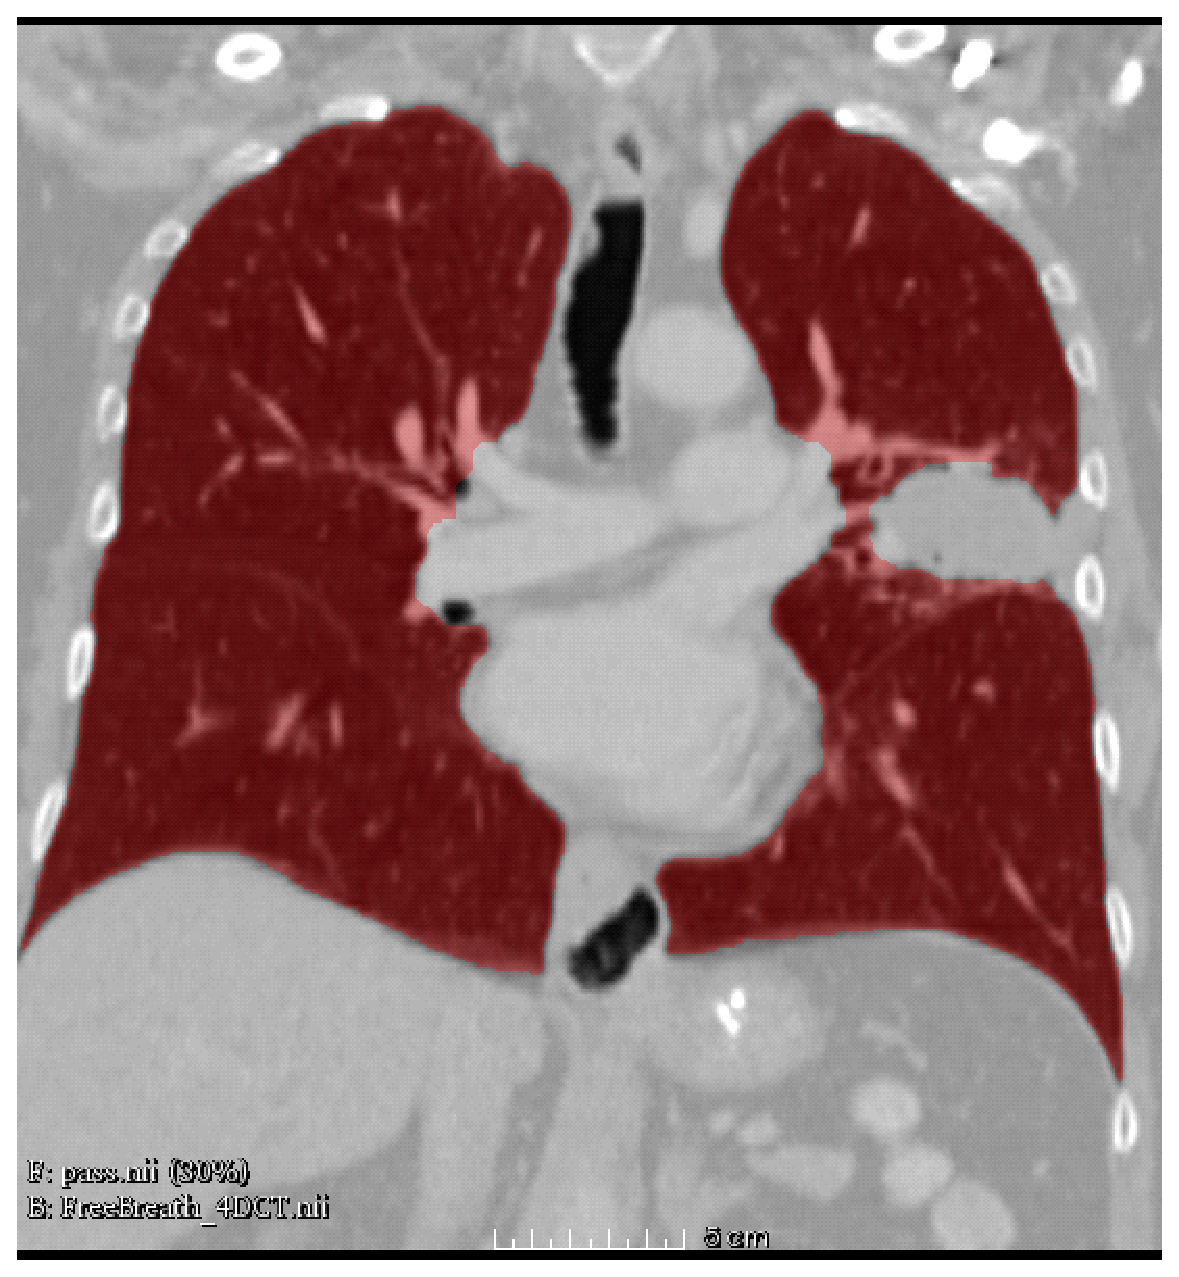
\includegraphics[width=1.08in]{figs/PFS-002_pass}
    \label{fig:PFS-002_pass}
    }
    \subfigure{
    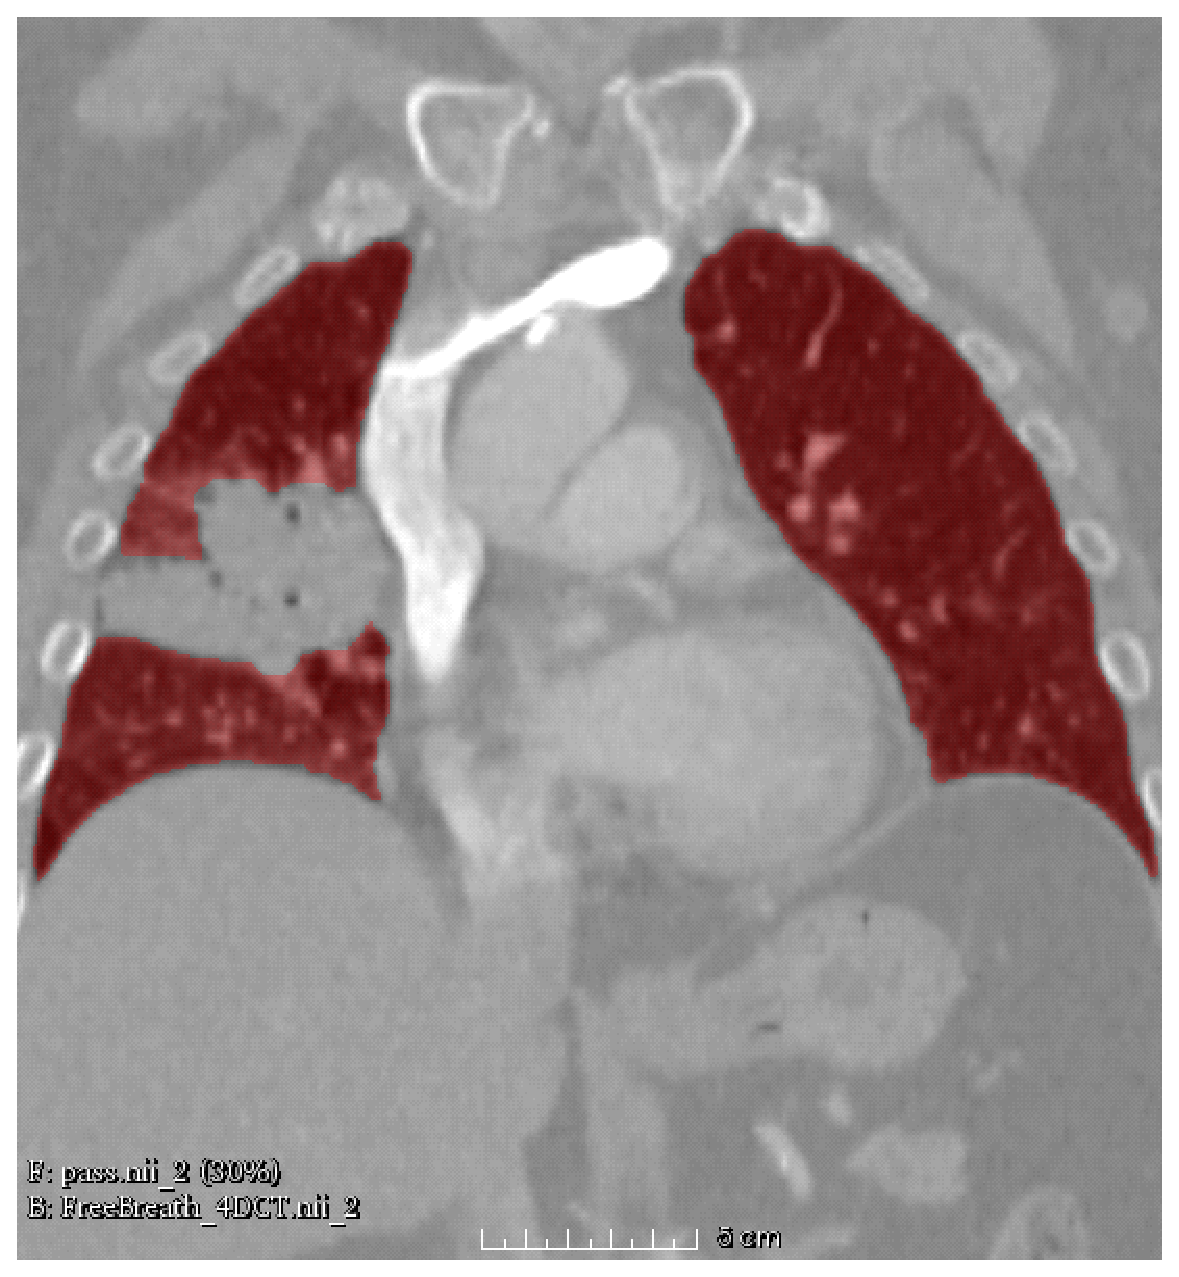
\includegraphics[width=1.08in]{figs/PFS-020_pass}
    \label{fig:PFS-020_pass}
    }
    \subfigure{
    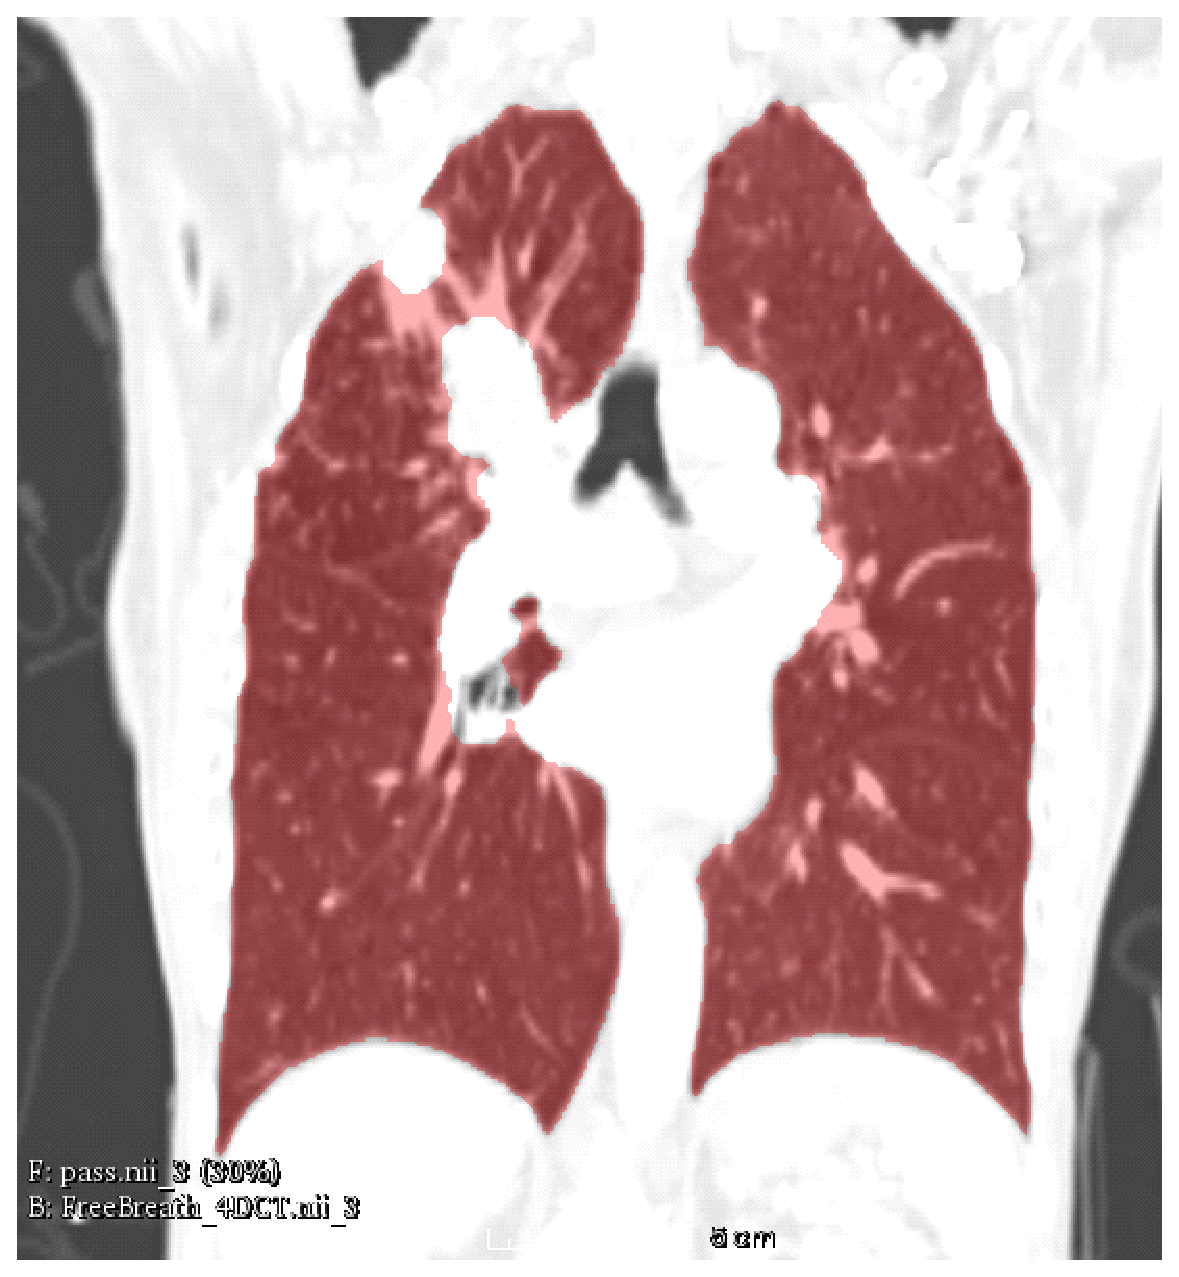
\includegraphics[width=1.08in]{figs/PFS-031_pass}
    \label{fig:PFS-031_pass}
    }
    \subfigure{
    \includegraphics[width=1.08in]{figs/PFS-032_pass}
    \label{fig:PFS-032_pass}
    }\\
    \subfigure{
    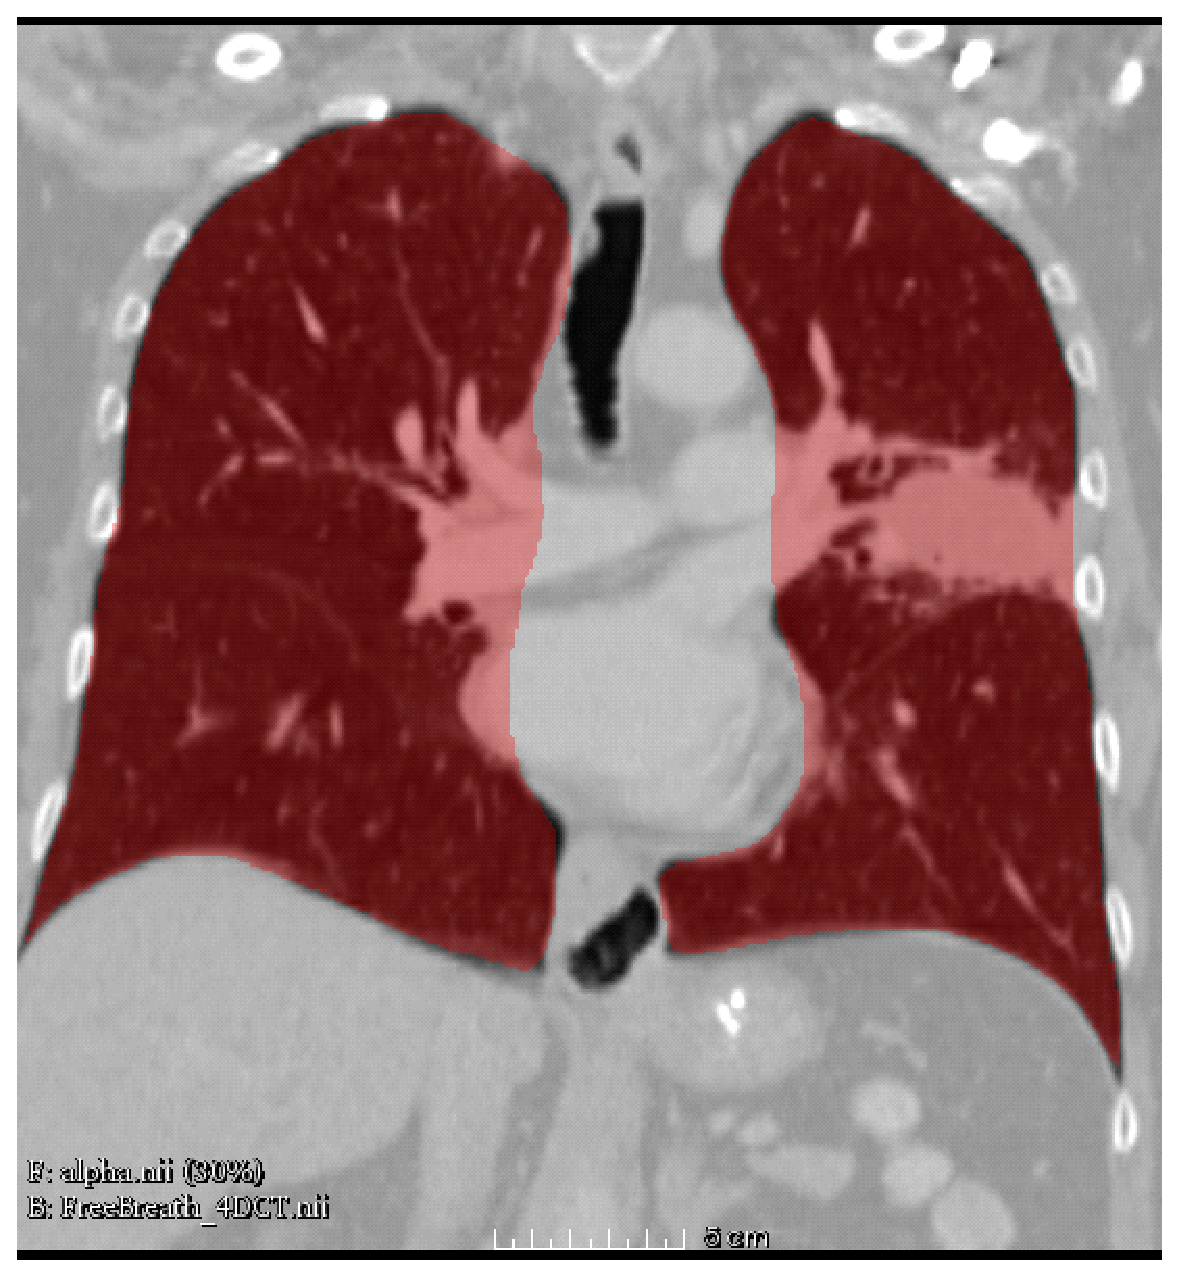
\includegraphics[width=1.08in]{figs/PFS-002_alpha}
    \label{fig:PFS-002_alpha}
    }
    \subfigure{
    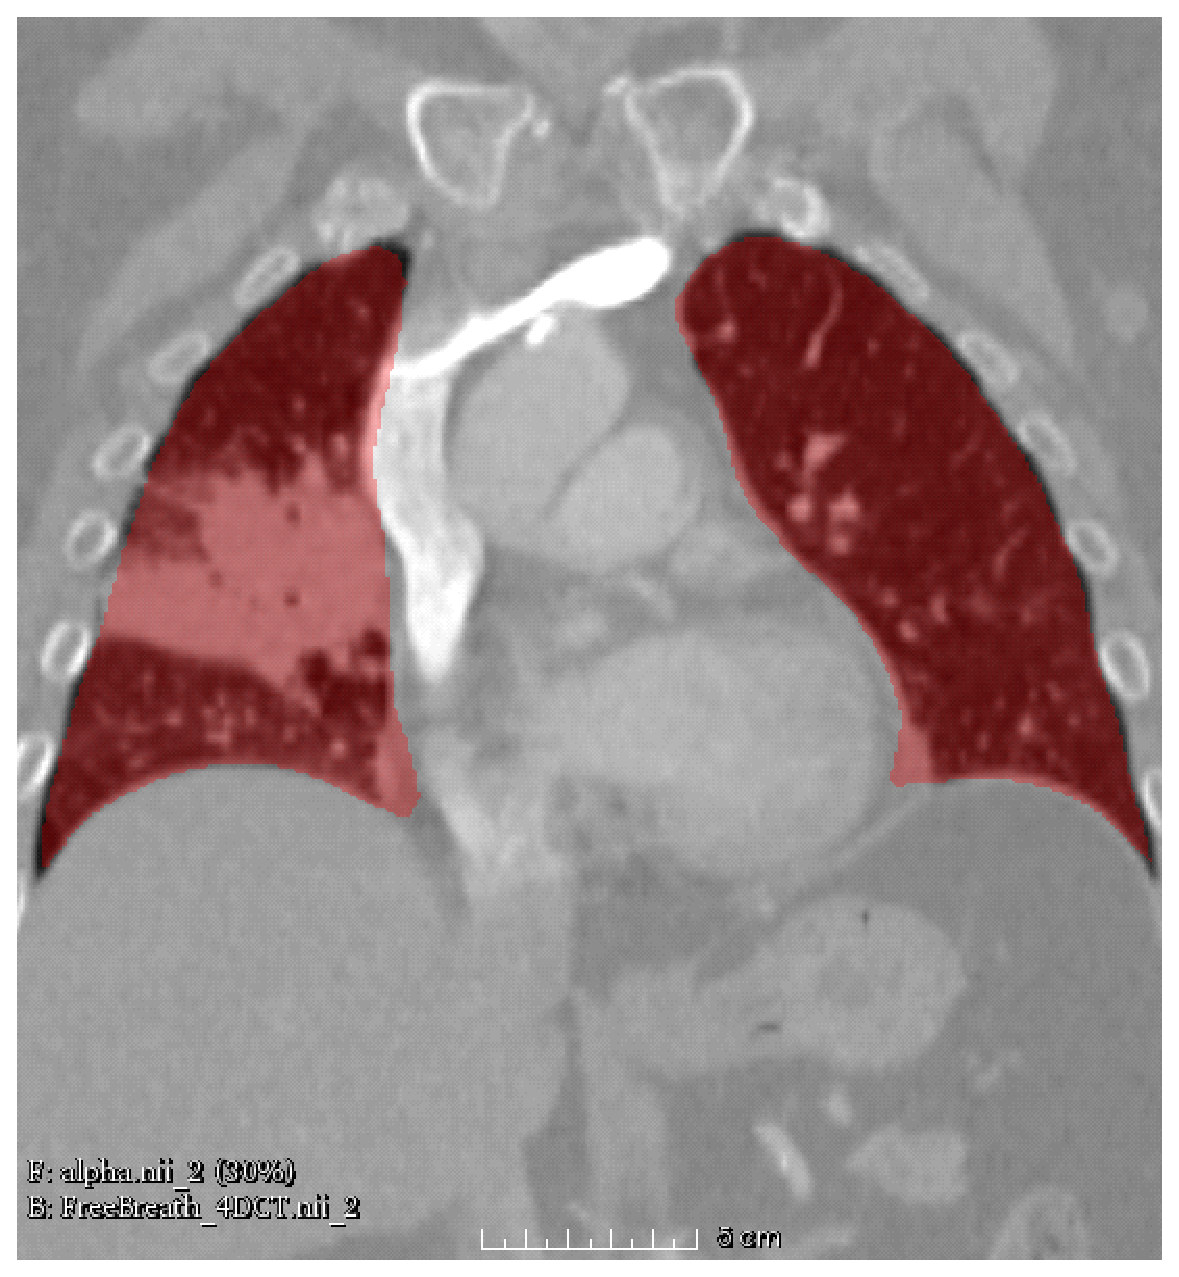
\includegraphics[width=1.08in]{figs/PFS-020_alpha}
    \label{fig:PFS-020_alpha}
    }
    \subfigure{
    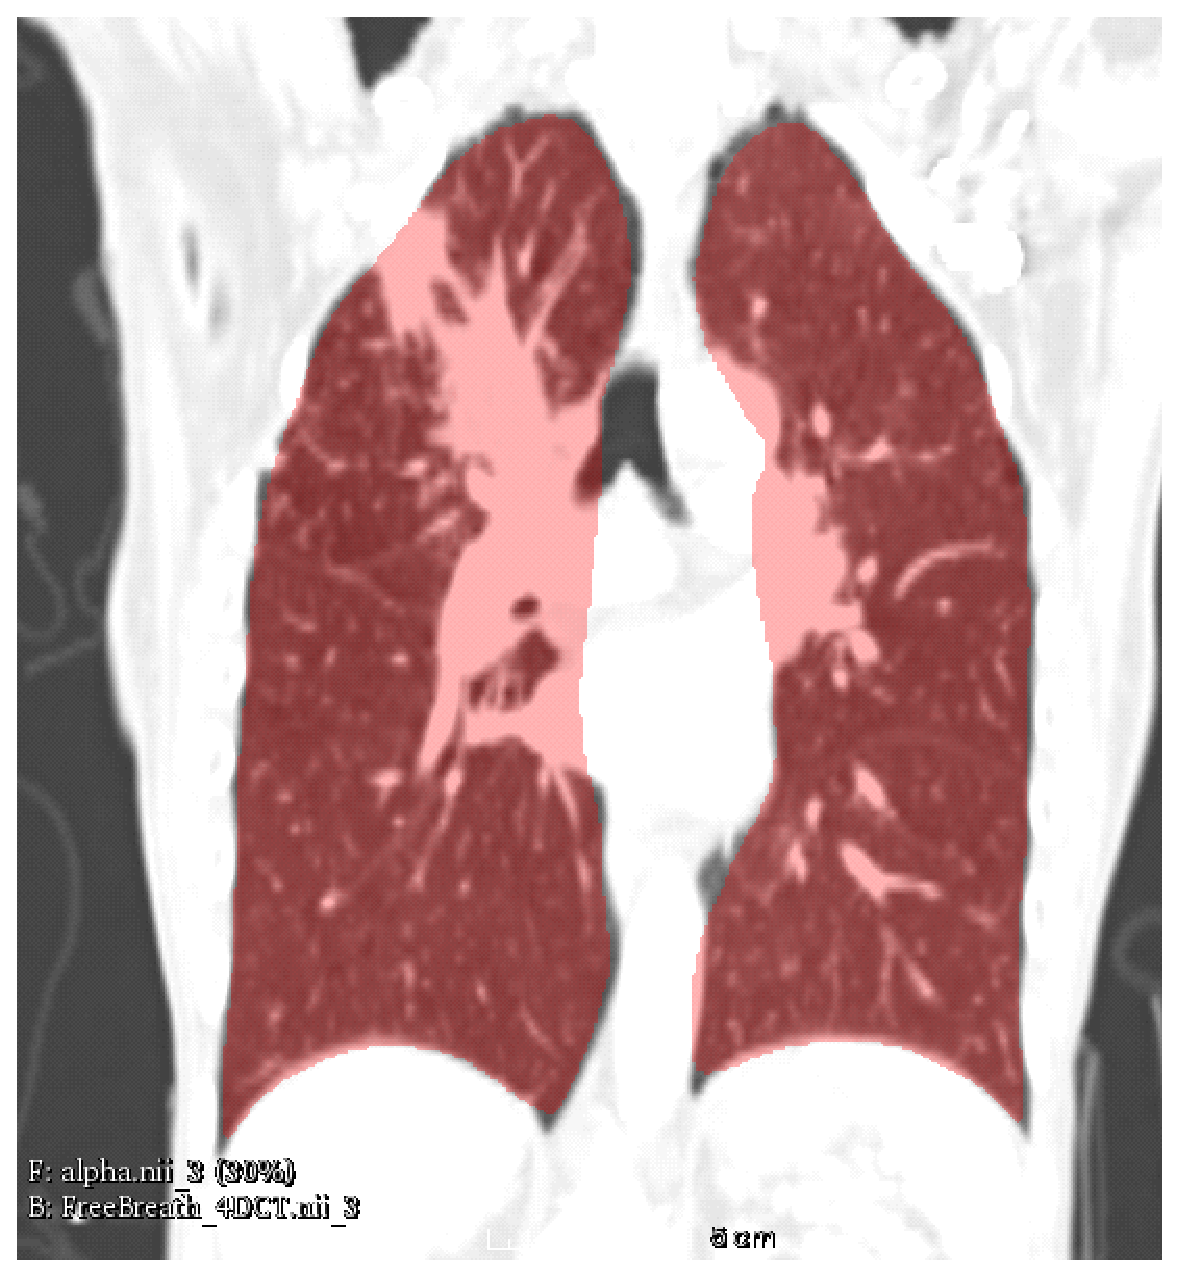
\includegraphics[width=1.08in]{figs/PFS-031_alpha}
    \label{fig:PFS-031_alpha}
    }
    \subfigure{
    \includegraphics[width=1.08in]{figs/PFS-032_alpha}
    \label{fig:PFS-032_alpha}
    }\\
    \subfigure{
    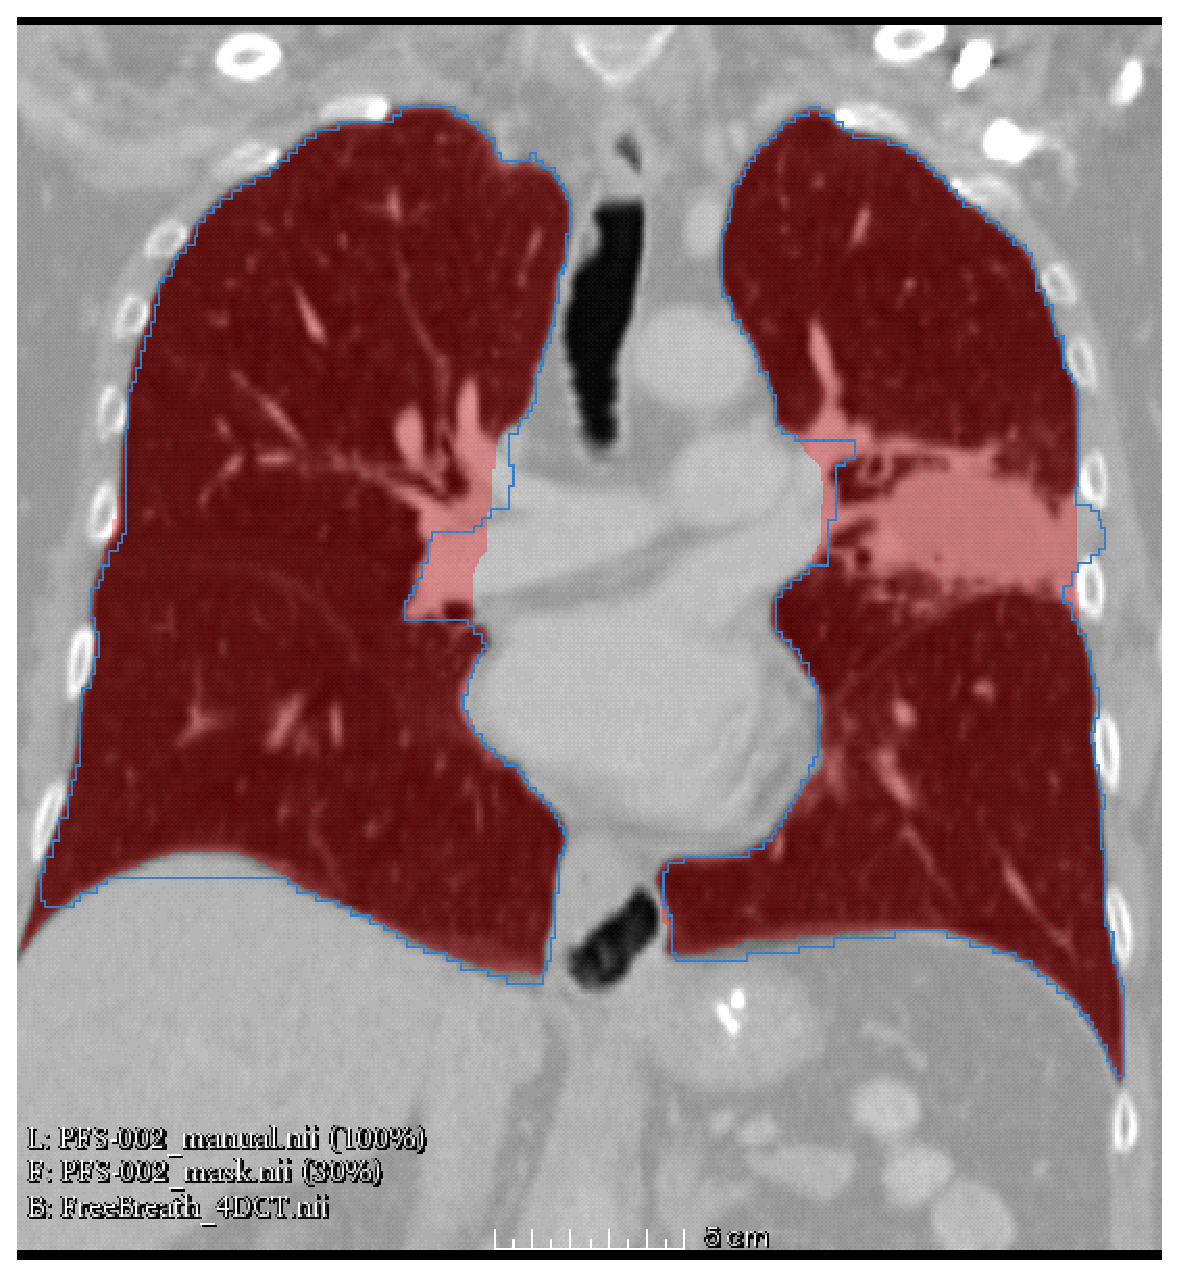
\includegraphics[width=1.08in]{figs/PFS-002_final}
    \label{fig:PFS-002_final}
    }
    \subfigure{
    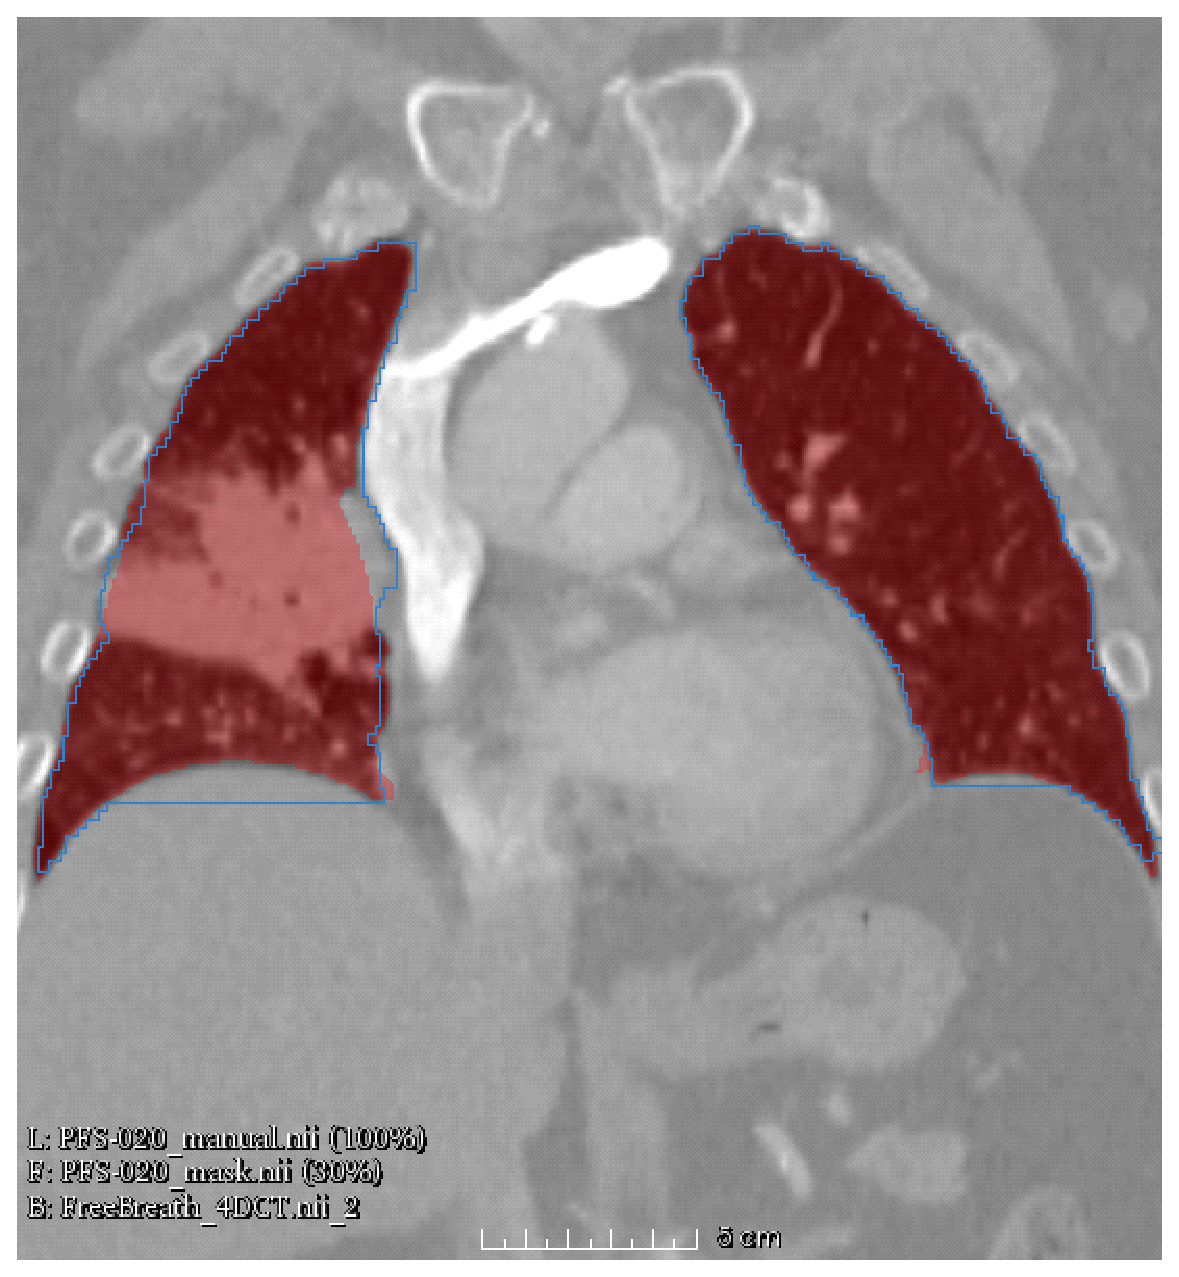
\includegraphics[width=1.08in]{figs/PFS-020_final}
    \label{fig:PFS-020_final}
    }
    \subfigure{
    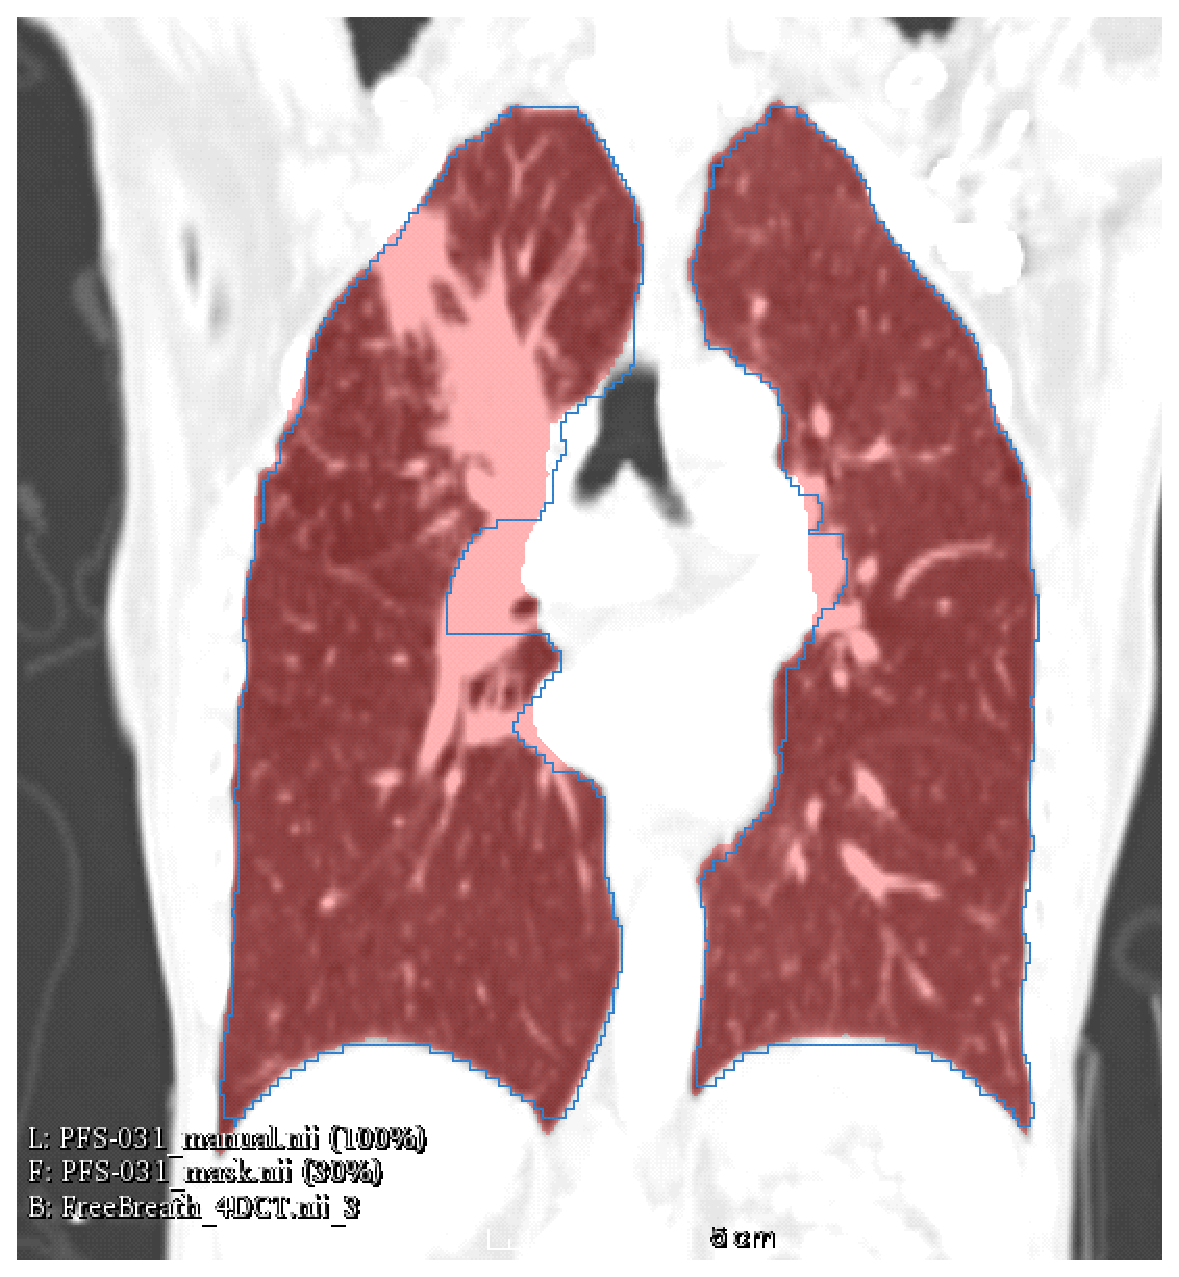
\includegraphics[width=1.08in]{figs/PFS-031_final}
    \label{fig:PFS-031_final}
    }
    \subfigure{
    \includegraphics[width=1.08in]{figs/PFS-032_final}
    \label{fig:PFS-032_final}
    }\\
    \subfigure{
    \includegraphics[width=1.08in]{figs/PFS-002_manual}
    \label{fig:PFS-002_manual}
    }
    \subfigure{
    \includegraphics[width=1.08in]{figs/PFS-020_manual}
    \label{fig:PFS-020_manual}
    }
    \subfigure{
    \includegraphics[width=1.08in]{figs/PFS-031_manual}
    \label{fig:PFS-031_manual}
    }
    \subfigure{
    \includegraphics[width=1.08in]{figs/PFS-032_manual}
    \label{fig:PFS-032_manual}
    }\\

    
    

  \caption{Segmentation at each step of the proposed method for
  four different data sets displayed in columns one to four. Row 1: CT image. Row 2: initial mask. Row 3: alpha shape of the initial mask. Row 4: final segmentation using the proposed automatic method. Row 5: manual segmentation.}
  \label{fig:resultseg}
\end{figure}




%
\section{Discussion}
%

The method shows good results with an average unsigned surface distance of 0.727 mm and an average DICE coefficient of 0.970 for all subjects. This surface distance is on the sub-voxel level. Additionally, we split the lungs into tumor and non-tumor groups. The DICE coefficient was 0.967 and 0.971 for tumor and non-tumor groups, respectively. The average unsigned surface distance was 0.758 mm and 0.702 mm for tumor and non-tumor groups, respectively. A t-test was performed to compare the surface distance error for lungs with tumors and lungs without tumors and no significant difference was found (p-value = 0.314). The surface distance for the initial mask was 1.368 mm and 0.710 mm for tumor and non-tumor groups, respectively. These results show that compared to the initial mask, our method significantly improves the average surface distance error for lungs with tumors (p-value 0.0008) and does not significantly change the average surface distance error for lungs without tumors (p-value 0.867).

By visual inspection, it is clear that the majority of discrepancy between our results and the manual segmentations occur at the mediastinum. This is a subjective region to segment, that can be observed on coronal slices of the manual segmentations. The manual segmentations were done on transverse slices and variation on where the mediastinal boundary was drawn between slices resulted in the boundary not being smooth in 3D. The proposed method produces a smooth mediastinum boundary that is consistent between subjects. 

In future work we plan on identifying the optimal $\alpha$ for each subject rather than using the same $\alpha$ for all subjects. Additionally, we plan to experiment with automatically identifying a spatially varying alpha to overcome over segmentation near mediastinum.

The experiments were run on a Linux machine with an Intel Xeon 2.27 GHz CPU and 48 GB of RAM. Generating the alpha shape and the graph search take approximately 13 and 1 minute(s) of computer time, respectively. The manual segmentation took on average 53 minutes per subject.
%
\section{Summary}
%
We proposed a method for segmentation of lungs in the presence of large tumors. The method utilizes an intensity based segmentation, alpha shapes correction, and a graph search framework final refinement.An average surface error distance of 0.727 mm and DICE coefficient of 0.970 and  were achieved. The accurate lung segmentation with  inclusion of tumor regions is valuable for radiation therapy treatment planning and further quantitative analysis.
%

\section{Acknowledgments}
%
This work was supported in part by 
%NIH grant CA166703.
XXXXXXX XXXXXXXXXXX.


%
% ---- Bibliography ----
%
\bibliography{refs.bib}
\bibliographystyle{splncs03}







\clearpage
\addtocmark[2]{Author Index} % additional numbered TOC entry
\renewcommand{\indexname}{Author Index}
\printindex
\clearpage
\iffalse
\addtocmark[2]{Subject Index} % additional numbered TOC entry
\markboth{Subject Index}{Subject Index}
\renewcommand{\indexname}{Subject Index}
%                                                           clmomu01.ind
%-----------------------------------------------------------------------
% CLMoMu01 1.0: LaTeX style files for books
% Sample index file for User's guide
% (c) Springer-Verlag HD
%-----------------------------------------------------------------------
\begin{theindex}
\item Absorption\idxquad 327
\item Absorption of radiation \idxquad 289--292,\, 299,\,300
\item Actinides \idxquad 244
\item Aharonov-Bohm effect\idxquad 142--146
\item Angular momentum\idxquad 101--112
\subitem algebraic treatment\idxquad 391--396
\item Angular momentum addition\idxquad 185--193
\item Angular momentum commutation relations\idxquad 101
\item Angular momentum quantization\idxquad 9--10,\,104--106
\item Angular momentum states\idxquad 107,\,321,\,391--396
\item Antiquark\idxquad 83
\item $\alpha$-rays\idxquad 101--103
\item Atomic theory\idxquad 8--10,\,219--249,\,327
\item Average value\newline ({\it see also\/} Expectation value)
15--16,\,25,\,34,\,37,\,357
\indexspace
\item Baker-Hausdorff formula\idxquad 23
\item Balmer formula\idxquad 8
\item Balmer series\idxquad 125
\item Baryon\idxquad 220,\,224
\item Basis\idxquad 98
\item Basis system\idxquad 164,\,376
\item Bell inequality\idxquad 379--381,\,382
\item Bessel functions\idxquad 201,\,313,\,337
\subitem spherical\idxquad 304--306,\, 309,\, 313--314,\,322
\item Bound state\idxquad 73--74,\,78--79,\,116--118,\,202,\, 267,\,
273,\,306,\,348,\,351
\item Boundary conditions\idxquad 59,\, 70
\item Bra\idxquad 159
\item Breit-Wigner formula\idxquad 80,\,84,\,332
\item Brillouin-Wigner perturbation theory\idxquad 203
\indexspace
\item Cathode rays\idxquad 8
\item Causality\idxquad 357--359
\item Center-of-mass frame\idxquad 232,\,274,\,338
\item Central potential\idxquad 113--135,\,303--314
\item Centrifugal potential\idxquad 115--116,\,323
\item Characteristic function\idxquad 33
\item Clebsch-Gordan coefficients\idxquad 191--193
\item Cold emission\idxquad 88
\item Combination principle, Ritz's\idxquad 124
\item Commutation relations\idxquad 27,\,44,\,353,\,391
\item Commutator\idxquad 21--22,\,27,\,44,\,344
\item Compatibility of measurements\idxquad 99
\item Complete orthonormal set\idxquad 31,\,40,\,160,\,360
\item Complete orthonormal system, {\it see}\newline
Complete orthonormal set
\item Complete set of observables, {\it see\/} Complete
set of operators
\indexspace
\item Eigenfunction\idxquad 34,\,46,\,344--346
\subitem radial\idxquad 321
\subsubitem calculation\idxquad 322--324
\item EPR argument\idxquad 377--378
\item Exchange term\idxquad 228,\,231,\,237,\,241,\,268,\,272
\indexspace
\item $f$-sum rule\idxquad 302
\item Fermi energy\idxquad 223
\indexspace
\item H$^+_2$ molecule\idxquad 26
\item Half-life\idxquad 65
\item Holzwarth energies\idxquad 68
\end{theindex}

\fi
\end{document}
